%%%%%%%%%%%%%%%%%%%%%%% file template.tex %%%%%%%%%%%%%%%%%%%%%%%%%
%
% This is a general template file for the LaTeX package SVJour3
% for Springer journals.          Springer Heidelberg 2010/09/16
%
% Copy it to a new file with a new name and use it as the basis
% for your article. Delete % signs as needed.
%
% This template includes a few options for different layouts and
% content for various journals. Please consult a previous issue of
% your journal as needed.
%
%%%%%%%%%%%%%%%%%%%%%%%%%%%%%%%%%%%%%%%%%%%%%%%%%%%%%%%%%%%%%%%%%%%
%
% First comes an example EPS file -- just ignore it and
% proceed on the \documentclass line
% your LaTeX will extract the file if required
\begin{filecontents*}{example.eps}
    %!PS-Adobe-3.0 EPSF-3.0
    %%BoundingBox: 19 19 221 221
    %%CreationDate: Mon Sep 29 1997
    %%Creator: programmed by hand (JK)
    %%EndComments
    gsave
    newpath
    20 20 moveto
    20 220 lineto
    220 220 lineto
    220 20 lineto
    closepath
    2 setlinewidth
    gsave
    .4 setgray fill
    grestore
    stroke
    grestore
\end{filecontents*}
%
\RequirePackage{fix-cm}
%
%\documentclass{svjour3}                     % onecolumn (standard format)
%\documentclass[smallcondensed]{svjour3}     % onecolumn (ditto)
%\documentclass[smallextended]{svjour3}       % onecolumn (second format)
\documentclass[smallextended,twocolumn]{svjour3}          % twocolumn
%
\journalname{Behavior Research Methods}
\smartqed  % flush right qed marks, e.g. at end of proof
%
\usepackage{graphicx}
%
%usepackage{mathptmx}      % use Times fonts if available on your TeX system
%
%\usepackage[natbibapa]{apacite}
\usepackage{natbib}


%\usepackage{tabularx}
\usepackage{amsmath}
\usepackage{textcomp}
\usepackage{booktabs}
\usepackage{units}
\usepackage[draft]{hyperref} %tmp added draft option for spilling refs
\usepackage{wrapfig}
\usepackage{todonotes}
\newcommand{\eg}{e.g., }
\newcommand{\ie}{i.e., }
\newcommand{\remodnav}{REMoDNaV}
\newcommand{\fig}[1]{{Figure~\ref{fig:#1}}}
\newcommand{\tab}[1]{{Table~\ref{tab:#1}}}
\newcommand{\param}[1]{{\texttt{#1}}}

\begin{document}

% #
% # %INCONSISTENCY Found label length mismatch between coders (MN, RA) for: TH34_img_vy_labelled_{}.mat
% #

% Truncate labels to shorter sample: [4990, 4988]
\newcommand{\imgMNRAMCLF}{6.1}
\newcommand{\imgMNRAMclfWOP}{3.0}
\newcommand{\imgMNRAFIXref}{70}
\newcommand{\imgMNRASACref}{9}
\newcommand{\imgMNRAPSOref}{21}
\newcommand{\imgMNRASPref}{0}
\newcommand{\imgMNRAFIXcod}{13}
\newcommand{\imgMNRASACcod}{15}
\newcommand{\imgMNRAPSOcod}{20}
\newcommand{\imgMNRASPcod}{53}
% ### img
% Comparison | MCLF | MCLFw/oP | Method | Fix | Sacc | PSO | SP
% --- | --- | --- | --- | --- | --- | --- | ---
% MN v RA | 6.1 | 3.0 | MN | 70 | 9 | 21 | 0
% -- | --  | -- | RA | 13 | 15 | 20 | 53
% #
% # %INCONSISTENCY Found label length mismatch between coders (MN, RA) for: UL27_trial17_labelled_{}.mat
% #

% Truncate labels to shorter sample: [454, 455]
\newcommand{\dotsMNRAMCLF}{10.7}
\newcommand{\dotsMNRAMclfWOP}{4.2}
\newcommand{\dotsMNRAFIXref}{11}
\newcommand{\dotsMNRASACref}{10}
\newcommand{\dotsMNRAPSOref}{9}
\newcommand{\dotsMNRASPref}{71}
\newcommand{\dotsMNRAFIXcod}{64}
\newcommand{\dotsMNRASACcod}{7}
\newcommand{\dotsMNRAPSOcod}{6}
\newcommand{\dotsMNRASPcod}{23}
% ### dots
% Comparison | MCLF | MCLFw/oP | Method | Fix | Sacc | PSO | SP
% --- | --- | --- | --- | --- | --- | --- | ---
% MN v RA | 10.7 | 4.2 | MN | 11 | 10 | 9 | 71
% -- | --  | -- | RA | 64 | 7 | 6 | 23
% #
% # %INCONSISTENCY Found label length mismatch between coders (MN, RA) for: TH38_video_dolphin_fov_labelled_{}.mat
% #

% Truncate labels to shorter sample: [4047, 4044]
% #
% # %INCONSISTENCY Found label length mismatch between coders (MN, RA) for: UL23_video_triple_jump_labelled_{}.mat
% #

% Truncate labels to shorter sample: [2823, 2821]
% #
% # %INCONSISTENCY Found label length mismatch between coders (MN, RA) for: UL27_video_triple_jump_labelled_{}.mat
% #

% Truncate labels to shorter sample: [2822, 2824]
\newcommand{\videoMNRAMCLF}{18.5}
\newcommand{\videoMNRAMclfWOP}{4.0}
\newcommand{\videoMNRAFIXref}{75}
\newcommand{\videoMNRASACref}{3}
\newcommand{\videoMNRAPSOref}{8}
\newcommand{\videoMNRASPref}{15}
\newcommand{\videoMNRAFIXcod}{16}
\newcommand{\videoMNRASACcod}{4}
\newcommand{\videoMNRAPSOcod}{3}
\newcommand{\videoMNRASPcod}{77}
% ### video
% Comparison | MCLF | MCLFw/oP | Method | Fix | Sacc | PSO | SP
% --- | --- | --- | --- | --- | --- | --- | ---
% MN v RA | 18.5 | 4.0 | MN | 75 | 3 | 8 | 15
% -- | --  | -- | RA | 16 | 4 | 3 | 77
\newcommand{\imgMNALMCLF}{23.1}
\newcommand{\imgMNALMclfWOP}{6.5}
\newcommand{\imgMNALFIXref}{86}
\newcommand{\imgMNALSACref}{2}
\newcommand{\imgMNALPSOref}{11}
\newcommand{\imgMNALSPref}{2}
\newcommand{\imgMNALFIXcod}{5}
\newcommand{\imgMNALSACcod}{13}
\newcommand{\imgMNALPSOcod}{6}
\newcommand{\imgMNALSPcod}{75}
% ### img
% Comparison | MCLF | MCLFw/oP | Method | Fix | Sacc | PSO | SP
% --- | --- | --- | --- | --- | --- | --- | ---
% MN v AL | 23.1 | 6.5 | MN | 86 | 2 | 11 | 2
% -- | --  | -- | AL | 5 | 13 | 6 | 75
\newcommand{\dotsMNALMCLF}{18.6}
\newcommand{\dotsMNALMclfWOP}{8.2}
\newcommand{\dotsMNALFIXref}{9}
\newcommand{\dotsMNALSACref}{5}
\newcommand{\dotsMNALPSOref}{8}
\newcommand{\dotsMNALSPref}{78}
\newcommand{\dotsMNALFIXcod}{77}
\newcommand{\dotsMNALSACcod}{6}
\newcommand{\dotsMNALPSOcod}{2}
\newcommand{\dotsMNALSPcod}{15}
% ### dots
% Comparison | MCLF | MCLFw/oP | Method | Fix | Sacc | PSO | SP
% --- | --- | --- | --- | --- | --- | --- | ---
% MN v AL | 18.6 | 8.2 | MN | 9 | 5 | 8 | 78
% -- | --  | -- | AL | 77 | 6 | 2 | 15
\newcommand{\videoMNALMCLF}{31.5}
\newcommand{\videoMNALMclfWOP}{7.9}
\newcommand{\videoMNALFIXref}{57}
\newcommand{\videoMNALSACref}{1}
\newcommand{\videoMNALPSOref}{6}
\newcommand{\videoMNALSPref}{36}
\newcommand{\videoMNALFIXcod}{36}
\newcommand{\videoMNALSACcod}{5}
\newcommand{\videoMNALPSOcod}{3}
\newcommand{\videoMNALSPcod}{55}
% ### video
% Comparison | MCLF | MCLFw/oP | Method | Fix | Sacc | PSO | SP
% --- | --- | --- | --- | --- | --- | --- | ---
% MN v AL | 31.5 | 7.9 | MN | 57 | 1 | 6 | 36
% -- | --  | -- | AL | 36 | 5 | 3 | 55
\newcommand{\imgRAALMCLF}{22.8}
\newcommand{\imgRAALMclfWOP}{6.4}
\newcommand{\imgRAALFIXref}{77}
\newcommand{\imgRAALSACref}{3}
\newcommand{\imgRAALPSOref}{11}
\newcommand{\imgRAALSPref}{9}
\newcommand{\imgRAALFIXcod}{13}
\newcommand{\imgRAALSACcod}{13}
\newcommand{\imgRAALPSOcod}{6}
\newcommand{\imgRAALSPcod}{68}
% ### img
% Comparison | MCLF | MCLFw/oP | Method | Fix | Sacc | PSO | SP
% --- | --- | --- | --- | --- | --- | --- | ---
% RA v AL | 22.8 | 6.4 | RA | 77 | 3 | 11 | 9
% -- | --  | -- | AL | 13 | 13 | 6 | 68
\newcommand{\dotsRAALMCLF}{22.8}
\newcommand{\dotsRAALMclfWOP}{10.8}
\newcommand{\dotsRAALFIXref}{28}
\newcommand{\dotsRAALSACref}{4}
\newcommand{\dotsRAALPSOref}{6}
\newcommand{\dotsRAALSPref}{61}
\newcommand{\dotsRAALFIXcod}{59}
\newcommand{\dotsRAALSACcod}{7}
\newcommand{\dotsRAALPSOcod}{2}
\newcommand{\dotsRAALSPcod}{31}
% ### dots
% Comparison | MCLF | MCLFw/oP | Method | Fix | Sacc | PSO | SP
% --- | --- | --- | --- | --- | --- | --- | ---
% RA v AL | 22.8 | 10.8 | RA | 28 | 4 | 6 | 61
% -- | --  | -- | AL | 59 | 7 | 2 | 31
\newcommand{\videoRAALMCLF}{28.5}
\newcommand{\videoRAALMclfWOP}{9.1}
\newcommand{\videoRAALFIXref}{38}
\newcommand{\videoRAALSACref}{3}
\newcommand{\videoRAALPSOref}{5}
\newcommand{\videoRAALSPref}{55}
\newcommand{\videoRAALFIXcod}{53}
\newcommand{\videoRAALSACcod}{6}
\newcommand{\videoRAALPSOcod}{5}
\newcommand{\videoRAALSPcod}{35}
% ### video
% Comparison | MCLF | MCLFw/oP | Method | Fix | Sacc | PSO | SP
% --- | --- | --- | --- | --- | --- | --- | ---
% RA v AL | 28.5 | 9.1 | RA | 38 | 3 | 5 | 55
% -- | --  | -- | AL | 53 | 6 | 5 | 35
\newcommand{\maxmclf}{10.8}
\newcommand{\FIXimgmnMN}{248}
\newcommand{\FIXimgmnRA}{242}
\newcommand{\FIXimgmnCDT}{397}
\newcommand{\FIXimgmnIDT}{399}
\newcommand{\FIXimgmnIKF}{174}
\newcommand{\FIXimgmnIMST}{304}
\newcommand{\FIXimgmnIHMM}{133}
\newcommand{\FIXimgmnIVT}{114}
\newcommand{\FIXimgmnNH}{258}
\newcommand{\FIXimgmnBIT}{209}
\newcommand{\FIXimgmnRE}{187}
\newcommand{\FIXimgsdMN}{271}
\newcommand{\FIXimgsdRA}{273}
\newcommand{\FIXimgsdCDT}{559}
\newcommand{\FIXimgsdIDT}{328}
\newcommand{\FIXimgsdIKF}{239}
\newcommand{\FIXimgsdIMST}{293}
\newcommand{\FIXimgsdIHMM}{216}
\newcommand{\FIXimgsdIVT}{204}
\newcommand{\FIXimgsdNH}{299}
\newcommand{\FIXimgsdBIT}{136}
\newcommand{\FIXimgsdRE}{132}
\newcommand{\FIXimgnoMN}{380}
\newcommand{\FIXimgnoRA}{369}
\newcommand{\FIXimgnoCDT}{251}
\newcommand{\FIXimgnoIDT}{242}
\newcommand{\FIXimgnoIKF}{513}
\newcommand{\FIXimgnoIMST}{333}
\newcommand{\FIXimgnoIHMM}{701}
\newcommand{\FIXimgnoIVT}{827}
\newcommand{\FIXimgnoNH}{292}
\newcommand{\FIXimgnoBIT}{423}
\newcommand{\FIXimgnoRE}{426}
\newcommand{\SACimgmnMN}{30}
\newcommand{\SACimgmnRA}{31}
\newcommand{\SACimgmnEM}{25}
\newcommand{\SACimgmnIDT}{35}
\newcommand{\SACimgmnIKF}{62}
\newcommand{\SACimgmnIMST}{17}
\newcommand{\SACimgmnIHMM}{48}
\newcommand{\SACimgmnIVT}{41}
\newcommand{\SACimgmnNH}{50}
\newcommand{\SACimgmnLNS}{29}
\newcommand{\SACimgmnRE}{39}
\newcommand{\SACimgsdMN}{17}
\newcommand{\SACimgsdRA}{15}
\newcommand{\SACimgsdEM}{22}
\newcommand{\SACimgsdIDT}{15}
\newcommand{\SACimgsdIKF}{37}
\newcommand{\SACimgsdIMST}{10}
\newcommand{\SACimgsdIHMM}{26}
\newcommand{\SACimgsdIVT}{22}
\newcommand{\SACimgsdNH}{20}
\newcommand{\SACimgsdLNS}{12}
\newcommand{\SACimgsdRE}{20}
\newcommand{\SACimgnoMN}{376}
\newcommand{\SACimgnoRA}{372}
\newcommand{\SACimgnoEM}{787}
\newcommand{\SACimgnoIDT}{258}
\newcommand{\SACimgnoIKF}{353}
\newcommand{\SACimgnoIMST}{335}
\newcommand{\SACimgnoIHMM}{368}
\newcommand{\SACimgnoIVT}{373}
\newcommand{\SACimgnoNH}{344}
\newcommand{\SACimgnoLNS}{390}
\newcommand{\SACimgnoRE}{388}
\newcommand{\PSOimgmnMN}{21}
\newcommand{\PSOimgmnRA}{21}
\newcommand{\PSOimgmnNH}{28}
\newcommand{\PSOimgmnLNS}{25}
\newcommand{\PSOimgmnRE}{19}
\newcommand{\PSOimgsdMN}{11}
\newcommand{\PSOimgsdRA}{9}
\newcommand{\PSOimgsdNH}{13}
\newcommand{\PSOimgsdLNS}{9}
\newcommand{\PSOimgsdRE}{8}
\newcommand{\PSOimgnoMN}{312}
\newcommand{\PSOimgnoRA}{309}
\newcommand{\PSOimgnoNH}{237}
\newcommand{\PSOimgnoLNS}{319}
\newcommand{\PSOimgnoRE}{277}
\newcommand{\PURimgmnMN}{363}
\newcommand{\PURimgmnRA}{305}
\newcommand{\PURimgmnRE}{197}
\newcommand{\PURimgsdMN}{187}
\newcommand{\PURimgsdRA}{184}
\newcommand{\PURimgsdRE}{73}
\newcommand{\PURimgnoMN}{3}
\newcommand{\PURimgnoRA}{16}
\newcommand{\PURimgnoRE}{118}
\newcommand{\rankFIXimgMN}{1}
\newcommand{\rankFIXimgRA}{0}
\newcommand{\rankFIXimgCDT}{10}
\newcommand{\rankFIXimgIDT}{7}
\newcommand{\rankFIXimgIKF}{5}
\newcommand{\rankFIXimgIMST}{3}
\newcommand{\rankFIXimgIHMM}{8}
\newcommand{\rankFIXimgIVT}{9}
\newcommand{\rankFIXimgNH}{2}
\newcommand{\rankFIXimgBIT}{4}
\newcommand{\rankFIXimgRE}{6}
\newcommand{\rankSACimgMN}{0}
\newcommand{\rankSACimgRA}{1}
\newcommand{\rankSACimgEM}{9}
\newcommand{\rankSACimgIDT}{3}
\newcommand{\rankSACimgIKF}{10}
\newcommand{\rankSACimgIMST}{6}
\newcommand{\rankSACimgIHMM}{8}
\newcommand{\rankSACimgIVT}{5}
\newcommand{\rankSACimgNH}{7}
\newcommand{\rankSACimgLNS}{2}
\newcommand{\rankSACimgRE}{4}
\newcommand{\rankPSOimgMN}{1}
\newcommand{\rankPSOimgRA}{0}
\newcommand{\rankPSOimgNH}{4}
\newcommand{\rankPSOimgLNS}{2}
\newcommand{\rankPSOimgRE}{3}
\newcommand{\rankPURimgMN}{1}
\newcommand{\rankPURimgRA}{0}
\newcommand{\rankPURimgRE}{2}
\newcommand{\FIXdotsmnMN}{161}
\newcommand{\FIXdotsmnRA}{131}
\newcommand{\FIXdotsmnCDT}{60}
\newcommand{\FIXdotsmnIDT}{323}
\newcommand{\FIXdotsmnIKF}{217}
\newcommand{\FIXdotsmnIMST}{268}
\newcommand{\FIXdotsmnIHMM}{214}
\newcommand{\FIXdotsmnIVT}{203}
\newcommand{\FIXdotsmnNH}{380}
\newcommand{\FIXdotsmnBIT}{189}
\newcommand{\FIXdotsmnRE}{116}
\newcommand{\FIXdotssdMN}{30}
\newcommand{\FIXdotssdRA}{99}
\newcommand{\FIXdotssdCDT}{127}
\newcommand{\FIXdotssdIDT}{146}
\newcommand{\FIXdotssdIKF}{184}
\newcommand{\FIXdotssdIMST}{140}
\newcommand{\FIXdotssdIHMM}{286}
\newcommand{\FIXdotssdIVT}{282}
\newcommand{\FIXdotssdNH}{333}
\newcommand{\FIXdotssdBIT}{113}
\newcommand{\FIXdotssdRE}{65}
\newcommand{\FIXdotsnoMN}{2}
\newcommand{\FIXdotsnoRA}{13}
\newcommand{\FIXdotsnoCDT}{165}
\newcommand{\FIXdotsnoIDT}{8}
\newcommand{\FIXdotsnoIKF}{72}
\newcommand{\FIXdotsnoIMST}{12}
\newcommand{\FIXdotsnoIHMM}{67}
\newcommand{\FIXdotsnoIVT}{71}
\newcommand{\FIXdotsnoNH}{30}
\newcommand{\FIXdotsnoBIT}{67}
\newcommand{\FIXdotsnoRE}{43}
\newcommand{\SACdotsmnMN}{23}
\newcommand{\SACdotsmnRA}{22}
\newcommand{\SACdotsmnEM}{17}
\newcommand{\SACdotsmnIDT}{32}
\newcommand{\SACdotsmnIKF}{60}
\newcommand{\SACdotsmnIMST}{13}
\newcommand{\SACdotsmnIHMM}{41}
\newcommand{\SACdotsmnIVT}{36}
\newcommand{\SACdotsmnNH}{43}
\newcommand{\SACdotsmnLNS}{26}
\newcommand{\SACdotsmnRE}{30}
\newcommand{\SACdotssdMN}{10}
\newcommand{\SACdotssdRA}{11}
\newcommand{\SACdotssdEM}{14}
\newcommand{\SACdotssdIDT}{14}
\newcommand{\SACdotssdIKF}{26}
\newcommand{\SACdotssdIMST}{5}
\newcommand{\SACdotssdIHMM}{17}
\newcommand{\SACdotssdIVT}{14}
\newcommand{\SACdotssdNH}{16}
\newcommand{\SACdotssdLNS}{11}
\newcommand{\SACdotssdRE}{13}
\newcommand{\SACdotsnoMN}{47}
\newcommand{\SACdotsnoRA}{47}
\newcommand{\SACdotsnoEM}{93}
\newcommand{\SACdotsnoIDT}{10}
\newcommand{\SACdotsnoIKF}{29}
\newcommand{\SACdotsnoIMST}{18}
\newcommand{\SACdotsnoIHMM}{27}
\newcommand{\SACdotsnoIVT}{28}
\newcommand{\SACdotsnoNH}{42}
\newcommand{\SACdotsnoLNS}{53}
\newcommand{\SACdotsnoRE}{40}
\newcommand{\PSOdotsmnMN}{15}
\newcommand{\PSOdotsmnRA}{15}
\newcommand{\PSOdotsmnNH}{24}
\newcommand{\PSOdotsmnLNS}{20}
\newcommand{\PSOdotsmnRE}{18}
\newcommand{\PSOdotssdMN}{5}
\newcommand{\PSOdotssdRA}{8}
\newcommand{\PSOdotssdNH}{12}
\newcommand{\PSOdotssdLNS}{9}
\newcommand{\PSOdotssdRE}{8}
\newcommand{\PSOdotsnoMN}{33}
\newcommand{\PSOdotsnoRA}{28}
\newcommand{\PSOdotsnoNH}{17}
\newcommand{\PSOdotsnoLNS}{31}
\newcommand{\PSOdotsnoRE}{14}
\newcommand{\PURdotsmnMN}{375}
\newcommand{\PURdotsmnRA}{378}
\newcommand{\PURdotsmnRE}{440}
\newcommand{\PURdotssdMN}{256}
\newcommand{\PURdotssdRA}{364}
\newcommand{\PURdotssdRE}{385}
\newcommand{\PURdotsnoMN}{37}
\newcommand{\PURdotsnoRA}{33}
\newcommand{\PURdotsnoRE}{34}
\newcommand{\rankFIXdotsMN}{1}
\newcommand{\rankFIXdotsRA}{0}
\newcommand{\rankFIXdotsCDT}{9}
\newcommand{\rankFIXdotsIDT}{5}
\newcommand{\rankFIXdotsIKF}{6}
\newcommand{\rankFIXdotsIMST}{3}
\newcommand{\rankFIXdotsIHMM}{8}
\newcommand{\rankFIXdotsIVT}{7}
\newcommand{\rankFIXdotsNH}{10}
\newcommand{\rankFIXdotsBIT}{4}
\newcommand{\rankFIXdotsRE}{2}
\newcommand{\rankSACdotsMN}{0}
\newcommand{\rankSACdotsRA}{1}
\newcommand{\rankSACdotsEM}{8}
\newcommand{\rankSACdotsIDT}{7}
\newcommand{\rankSACdotsIKF}{10}
\newcommand{\rankSACdotsIMST}{6}
\newcommand{\rankSACdotsIHMM}{9}
\newcommand{\rankSACdotsIVT}{4}
\newcommand{\rankSACdotsNH}{5}
\newcommand{\rankSACdotsLNS}{2}
\newcommand{\rankSACdotsRE}{3}
\newcommand{\rankPSOdotsMN}{0}
\newcommand{\rankPSOdotsRA}{1}
\newcommand{\rankPSOdotsNH}{4}
\newcommand{\rankPSOdotsLNS}{2}
\newcommand{\rankPSOdotsRE}{3}
\newcommand{\rankPURdotsMN}{1}
\newcommand{\rankPURdotsRA}{0}
\newcommand{\rankPURdotsRE}{2}
\newcommand{\FIXvideomnMN}{318}
\newcommand{\FIXvideomnRA}{240}
\newcommand{\FIXvideomnCDT}{213}
\newcommand{\FIXvideomnIDT}{554}
\newcommand{\FIXvideomnIKF}{228}
\newcommand{\FIXvideomnIMST}{526}
\newcommand{\FIXvideomnIHMM}{234}
\newcommand{\FIXvideomnIVT}{202}
\newcommand{\FIXvideomnNH}{429}
\newcommand{\FIXvideomnBIT}{248}
\newcommand{\FIXvideomnRE}{147}
\newcommand{\FIXvideosdMN}{289}
\newcommand{\FIXvideosdRA}{189}
\newcommand{\FIXvideosdCDT}{297}
\newcommand{\FIXvideosdIDT}{454}
\newcommand{\FIXvideosdIKF}{296}
\newcommand{\FIXvideosdIMST}{825}
\newcommand{\FIXvideosdIHMM}{319}
\newcommand{\FIXvideosdIVT}{306}
\newcommand{\FIXvideosdNH}{336}
\newcommand{\FIXvideosdBIT}{215}
\newcommand{\FIXvideosdRE}{107}
\newcommand{\FIXvideonoMN}{67}
\newcommand{\FIXvideonoRA}{67}
\newcommand{\FIXvideonoCDT}{211}
\newcommand{\FIXvideonoIDT}{48}
\newcommand{\FIXvideonoIKF}{169}
\newcommand{\FIXvideonoIMST}{71}
\newcommand{\FIXvideonoIHMM}{194}
\newcommand{\FIXvideonoIVT}{227}
\newcommand{\FIXvideonoNH}{83}
\newcommand{\FIXvideonoBIT}{170}
\newcommand{\FIXvideonoRE}{144}
\newcommand{\SACvideomnMN}{26}
\newcommand{\SACvideomnRA}{25}
\newcommand{\SACvideomnEM}{20}
\newcommand{\SACvideomnIDT}{24}
\newcommand{\SACvideomnIKF}{55}
\newcommand{\SACvideomnIMST}{18}
\newcommand{\SACvideomnIHMM}{42}
\newcommand{\SACvideomnIVT}{36}
\newcommand{\SACvideomnNH}{44}
\newcommand{\SACvideomnLNS}{28}
\newcommand{\SACvideomnRE}{33}
\newcommand{\SACvideosdMN}{13}
\newcommand{\SACvideosdRA}{12}
\newcommand{\SACvideosdEM}{16}
\newcommand{\SACvideosdIDT}{53}
\newcommand{\SACvideosdIKF}{20}
\newcommand{\SACvideosdIMST}{10}
\newcommand{\SACvideosdIHMM}{18}
\newcommand{\SACvideosdIVT}{16}
\newcommand{\SACvideosdNH}{18}
\newcommand{\SACvideosdLNS}{12}
\newcommand{\SACvideosdRE}{15}
\newcommand{\SACvideonoMN}{116}
\newcommand{\SACvideonoRA}{126}
\newcommand{\SACvideonoEM}{252}
\newcommand{\SACvideonoIDT}{41}
\newcommand{\SACvideonoIKF}{107}
\newcommand{\SACvideonoIMST}{76}
\newcommand{\SACvideonoIHMM}{109}
\newcommand{\SACvideonoIVT}{112}
\newcommand{\SACvideonoNH}{1104}
\newcommand{\SACvideonoLNS}{122}
\newcommand{\SACvideonoRE}{118}
\newcommand{\PSOvideomnMN}{20}
\newcommand{\PSOvideomnRA}{17}
\newcommand{\PSOvideomnNH}{28}
\newcommand{\PSOvideomnLNS}{24}
\newcommand{\PSOvideomnRE}{18}
\newcommand{\PSOvideosdMN}{11}
\newcommand{\PSOvideosdRA}{8}
\newcommand{\PSOvideosdNH}{13}
\newcommand{\PSOvideosdLNS}{10}
\newcommand{\PSOvideosdRE}{8}
\newcommand{\PSOvideonoMN}{97}
\newcommand{\PSOvideonoRA}{89}
\newcommand{\PSOvideonoNH}{78}
\newcommand{\PSOvideonoLNS}{87}
\newcommand{\PSOvideonoRE}{86}
\newcommand{\PURvideomnMN}{521}
\newcommand{\PURvideomnRA}{472}
\newcommand{\PURvideomnRE}{314}
\newcommand{\PURvideosdMN}{347}
\newcommand{\PURvideosdRA}{319}
\newcommand{\PURvideosdRE}{229}
\newcommand{\PURvideonoMN}{50}
\newcommand{\PURvideonoRA}{68}
\newcommand{\PURvideonoRE}{97}
\newcommand{\rankFIXvideoMN}{0}
\newcommand{\rankFIXvideoRA}{1}
\newcommand{\rankFIXvideoCDT}{7}
\newcommand{\rankFIXvideoIDT}{8}
\newcommand{\rankFIXvideoIKF}{4}
\newcommand{\rankFIXvideoIMST}{10}
\newcommand{\rankFIXvideoIHMM}{6}
\newcommand{\rankFIXvideoIVT}{9}
\newcommand{\rankFIXvideoNH}{2}
\newcommand{\rankFIXvideoBIT}{3}
\newcommand{\rankFIXvideoRE}{5}
\newcommand{\rankSACvideoMN}{0}
\newcommand{\rankSACvideoRA}{1}
\newcommand{\rankSACvideoEM}{6}
\newcommand{\rankSACvideoIDT}{9}
\newcommand{\rankSACvideoIKF}{8}
\newcommand{\rankSACvideoIMST}{4}
\newcommand{\rankSACvideoIHMM}{7}
\newcommand{\rankSACvideoIVT}{5}
\newcommand{\rankSACvideoNH}{10}
\newcommand{\rankSACvideoLNS}{2}
\newcommand{\rankSACvideoRE}{3}
\newcommand{\rankPSOvideoMN}{1}
\newcommand{\rankPSOvideoRA}{2}
\newcommand{\rankPSOvideoNH}{4}
\newcommand{\rankPSOvideoLNS}{3}
\newcommand{\rankPSOvideoRE}{0}
\newcommand{\rankPURvideoMN}{1}
\newcommand{\rankPURvideoRA}{0}
\newcommand{\rankPURvideoRE}{2}
% #
% # %INCONSISTENCY Found label length mismatch between coders for: TH34_img_vy_labelled_{}.mat
% #

% Truncate labels to shorter sample: 4988
\newcommand{\kappaRAMNimgFix}{0.84}
\newcommand{\kappaALRAimgFix}{0.55}
\newcommand{\kappaALMNimgFix}{0.52}
% #
% # %INCONSISTENCY Found label length mismatch between coders for: TH34_img_vy_labelled_{}.mat
% #

% Truncate labels to shorter sample: 4988
\newcommand{\kappaRAMNimgSac}{0.91}
\newcommand{\kappaALRAimgSac}{0.78}
\newcommand{\kappaALMNimgSac}{0.78}
% #
% # %INCONSISTENCY Found label length mismatch between coders for: TH34_img_vy_labelled_{}.mat
% #

% Truncate labels to shorter sample: 4988
\newcommand{\kappaRAMNimgPSO}{0.76}
\newcommand{\kappaALRAimgPSO}{0.59}
\newcommand{\kappaALMNimgPSO}{0.58}
% #
% # %INCONSISTENCY Found label length mismatch between coders for: UL27_trial17_labelled_{}.mat
% #

% Truncate labels to shorter sample: 454
\newcommand{\kappaRAMNdotsFix}{0.65}
\newcommand{\kappaALRAdotsFix}{0.37}
\newcommand{\kappaALMNdotsFix}{0.45}
% #
% # %INCONSISTENCY Found label length mismatch between coders for: UL27_trial17_labelled_{}.mat
% #

% Truncate labels to shorter sample: 454
\newcommand{\kappaRAMNdotsSac}{0.81}
\newcommand{\kappaALRAdotsSac}{0.72}
\newcommand{\kappaALMNdotsSac}{0.78}
% #
% # %INCONSISTENCY Found label length mismatch between coders for: UL27_trial17_labelled_{}.mat
% #

% Truncate labels to shorter sample: 454
\newcommand{\kappaRAMNdotsPSO}{0.62}
\newcommand{\kappaALRAdotsPSO}{0.38}
\newcommand{\kappaALMNdotsPSO}{0.41}
% #
% # %INCONSISTENCY Found label length mismatch between coders for: TH38_video_dolphin_fov_labelled_{}.mat
% #

% Truncate labels to shorter sample: 4044
% #
% # %INCONSISTENCY Found label length mismatch between coders for: UL23_video_triple_jump_labelled_{}.mat
% #

% Truncate labels to shorter sample: 2821
% #
% # %INCONSISTENCY Found label length mismatch between coders for: UL27_video_triple_jump_labelled_{}.mat
% #

% Truncate labels to shorter sample: 2822
\newcommand{\kappaRAMNvideoFix}{0.65}
\newcommand{\kappaALRAvideoFix}{0.44}
\newcommand{\kappaALMNvideoFix}{0.39}
% #
% # %INCONSISTENCY Found label length mismatch between coders for: TH38_video_dolphin_fov_labelled_{}.mat
% #

% Truncate labels to shorter sample: 4044
% #
% # %INCONSISTENCY Found label length mismatch between coders for: UL23_video_triple_jump_labelled_{}.mat
% #

% Truncate labels to shorter sample: 2821
% #
% # %INCONSISTENCY Found label length mismatch between coders for: UL27_video_triple_jump_labelled_{}.mat
% #

% Truncate labels to shorter sample: 2822
\newcommand{\kappaRAMNvideoSac}{0.87}
\newcommand{\kappaALRAvideoSac}{0.76}
\newcommand{\kappaALMNvideoSac}{0.79}
% #
% # %INCONSISTENCY Found label length mismatch between coders for: TH38_video_dolphin_fov_labelled_{}.mat
% #

% Truncate labels to shorter sample: 4044
% #
% # %INCONSISTENCY Found label length mismatch between coders for: UL23_video_triple_jump_labelled_{}.mat
% #

% Truncate labels to shorter sample: 2821
% #
% # %INCONSISTENCY Found label length mismatch between coders for: UL27_video_triple_jump_labelled_{}.mat
% #

% Truncate labels to shorter sample: 2822
\newcommand{\kappaRAMNvideoPSO}{0.65}
\newcommand{\kappaALRAvideoPSO}{0.45}
\newcommand{\kappaALMNvideoPSO}{0.51}


\onecolumn
\title{REMoDNaV: Robust Eye Movement Detection for Natural Viewing } %\\ (remodnav)

% \titlenote{The title should be detailed enough for someone to know whether
% the article would be of interest to them, but also concise. Please ensure the
% broadness and claims within the title are appropriate to the content of the
% article itself.}

\author{%
  Asim~H.~Dar\textsuperscript{*} \and
Adina~Wagner\textsuperscript{*} \and
Michael~Hanke\\
{\small \textsuperscript{*} Both authors have contributed equally}}

\institute{Asim~H.~Dar \at
Special Lab Non-Invasive Brain Imaging, Leibniz Institute for Neurobiology, Brenneckestra{\ss}e~6, Magde\-burg, Germany
%Tel.: +123-45-678910\\
%Fax: +123-45-678910\\
%\email{fauthor@example.com}           %  \\
%             \emph{Present address:} of F. Author  %  if needed
\and
Adina Wagner \at
Psychoinformatics lab, Institute of Neuroscience and Medicine (INM-7: Brain and Behaviour), Research Centre Jülich, Germany
\and
Michael Hanke \at
Psychoinformatics lab, Institute of Neuroscience and Medicine (INM-7: Brain and Behaviour), Research Centre Jülich and Institute of Systems Neuroscience
Heinrich Heine University Düsseldorf, Germany
\email{michael.hanke@gmail.com}
}


%\affil[1]{Psychoinformatics Lab, Institute of Psychology, Otto-von-Guericke University, Magdeburg, Germany}

\date{Received: date / Accepted: date}

\maketitle

% Please list all authors that played a significant role in the research
% involved in the article. Please provide full affiliation information
% (including full institutional address, ZIP code and e-mail address) for all
% authors, and identify who is/are the corresponding author(s).

\begin{abstract}

% Abstracts should be up to 300 words and provide a succinct summary of the
% article. Although the abstract should explain why the article might be
% interesting, care should be taken not to inappropriately over-emphasize the
% importance of the work described in the article. Citations should not be used
% in the abstract, and the use of abbreviations should be minimized. If you are
% writing a Research or Systematic Review article, please structure your
% abstract into Background, Methods, Results, and Conclusions.

% general intro
Tracking of eye movements is an established measurement for many types of
experimental paradigms.
% targeted intro
More complex and lengthier visual stimuli have made algorithmic approaches to
eye movement event detection the most pragmatic option.
% problem statement
A recent analysis revealed that many current algorithms are lackluster when it
comes to data from viewing dynamic stimuli such as video sequences.
% out contribution
Here we present an event detection algorithm---built on an existing
velocity-based approach---that is suitable for both static and dynamic
stimulation, and is capable of detecting saccades, post-saccadic
oscillations, fixations, and smooth pursuit events.
% results
We validated detection performance and robustness on three public datasets:
1)~manually annotated, trial-based gaze trajectories for viewing static images,
moving dots, and short video sequences, 2)~lab-quality gaze recordings for a
feature length movie, and 3)~gaze recordings acquired under suboptimal lighting
conditions inside the bore of a magnetic resonance imaging (MRI) scanner for
the same full-length movie.
%
We found that the proposed algorithm performs on par or better compared
to state-of-the-art alternatives for static stimulation. Moreover, it yields
eye movement events with biologically plausible characteristics on prolonged
recordings without a trial-structure. Lastly, algorithm performance is robust
on data acquired under suboptimal conditions that exhibit a temporally
varying noise level.
% general context
These results indicate that the proposed algorithm is a robust tool with
improved detection accuracy across a range of use cases.
% broader perspective
A cross-platform compatible implementation in the Python programming language
is available as free and open source software.

\keywords{%
eye tracking \and
adaptive detection algorithm \and
saccade detection algorithm \and
statistical saccade analysis \and
glissade detection \and
adaptive threshold algorithm \and
data preprocessing
}
\end{abstract}

% \todo[inline]{The scope of the article is a "Data Note" that describes new
% "derived" data generated from the raw eyetracking data released by the
% studyforrest project. I propose to produce two types of artifacts: 1.
% filtered/preprocessed eyetracking data, and 2. a list with detected saccades
% for each recording.}

% \todo[inline]{It would be good to also release fully preprocessed data. Apart
% from applying the chosen filter, it would also make sense to me to temporally
% down-sample the data. What would be a practical sampling rate that reduces
% the data size (and some noise), but does not negatively impact most potential
% analyses? 100 Hz? 200 Hz? Even in the latter case it would still be a 5x
% reduction in size.}

% \todo[inline, backgroundcolor = green]{250 Hz is the lower limit to detect
% most saccades (Kern 2000). However,the downsampled data did not reach the
% same accuracy level as the higher frequency data, probably because the
% algorithm was designed to work on higher frequencies (as stated by the
% authors). Therefore we left it at the 1000 Hz frequency}

\twocolumn
\section*{Introduction}\label{intro}

% \todo[inline]{\textit{make connection to studyforrest. studyforrest has
% eyetracking data. why is it necessary to have that preprocessed?}}

% The data used for this thesis originates from the open science project
% 'studyforrest'. It centers around two large data acquisition phases employing
% the movie 'Forrest Gump' as stimulus. \cite{Hanke.2014,Hanke.2016} The
% project provides a large variety of collections of data to enable fellow
% researchers to build upon existing knowledge and further extend the dataset.
% Along other measures, the eye gaze coordinates were being recorded during the
% original sessions. Contrarily to the standard automatic detection process we
% applied an adaptive algorithm to the eye movement data to provide a more
% precise computation of saccades and fixations.

A spreading theme in cognitive neuroscience is to use dynamic and natural
stimuli as opposed to isolated and distinct imagery \citep{real_world}. Using
dynamic stimuli promises to observe the nuances of cognition in a more natural
environment. Some interesting applications include the determination of neural
response to changes in facial expression \citep{Harris2014}, understanding
complex social interactions by using videos \citep{Tikka2012} and more
untouched themes such as the underlying processing of music
\citep{Toiviainen2014}. In such studies, an unobtrusive behavioral measurement
is required to quantify the relationship between stimulus and response.
Tracking the focus of participants' gaze is a suitable, well established
measure that has been successfully employed in a variety of studies ranging
from the understanding of visual attention \citep{HantaoLiu2011}, memory
\citep{Hannula2010} and language comprehension \citep{Gordon2006}.
%
Regardless of use case, the raw eye tracking data (position coordinates)
provided by eye tracking devices are rarely used ``as is". Instead, in order
to disentangle different cognitive, occulomotor, or perceptive states
associated with different types of eye movements, most research relies on the
classification of eye gaze data into distinct eye movement event categories
\citep{Schutz2011}. The most feasible approach for doing this lies in the
application of appropriate event detection algorithms.

However, a recent comparison of algorithms found that while many readily
available algorithms for eye movement classification performed well on data
from static stimulation or short trial-based acquisitions with simplified
moving stimuli, none worked particularly well on data from complex natural
dynamic stimulation, such as video clips, when compared to human coders
\citep{Andersson2017}.
%
And indeed, when we evaluated an algorithm by \citet{Nystrom2010AnData}, one of
the winners in the aforementioned comparison, on data from prolonged
stimulation (\unit[$\approx$15]{min}) with a feature film, we found the
average and median durations of labeled fixations to exceeded literature
reports \citep[\eg][]{holmqvist2011eye,dorr2010variability} by up to a factor
of two.  Additionally, and in particular for increasing levels of noise in the
data, the algorithm classified too few fixations, as also noted by
\citet{Friedman2018}, because it discarded potential fixation events that
contained artifacts such as blinks.
%
However, robust performance on noisy data is of particular relevance in the
context of ``natural stimulation'', as the ultimate natural stimulation is the
actual natural environment, and data acquired outdoors or with mobile
devices typically does not match the quality achieved in dedicated lab
setups.

Therefore our objective was to improve upon the available eye movement
detection and classification algorithms, and develop a tool that performs
robustly on data from dynamic natural stimulation, without sacrificing detection
accuracy for static and simplified stimulation. Importantly, we aimed for
applicability to prolonged recordings that lack any kind of trial structure,
and exhibit periods of signal-loss and non-stationary noise levels.
% maybe work in \citep{Hooge2018} again
In addition to the event categories \textit{fixation}, \textit{saccade}, and
\textit{post-saccadic oscillation} (PSO; sometimes termed ``glissade"), the
algorithm had to support the detection of \textit{smooth pursuit} events, as
emphasized by \cite{Friedman2018}.  These are slow movements of the eye during
tracking of a moving target and are routinely evoked by moving visual objects
during dynamic stimulation \citep{carl1987pursuits}.  If this type of eye
movement is not properly detected and labeled, erroneous fixation and saccade
events (which smooth pursuits would be classified into instead) are introduced.
Contemporary algorithms rarely provide this functionality (but see \eg
\cite[but see \eg][]{LARSSON2015145,Komogortsev2013} for existing algorithms with
smooth pursuit detection).

Here we introduce \remodnav\ (robust eye movement detection for natural
viewing), a novel tool that aims to meet these objectives. It is built on the
aforementioned algorithm by \citet{Nystrom2010AnData} (subsequently labeled NH)
that employs an adaptive approach to velocity based eye movement event
detection and classification. \remodnav\ enhances NH with the use of robust
statistics, and a compartmentalization of prolonged time series into short,
more homogeneous segments with more uniform noise levels. Furthermore, it adds
support for pursuit event detection. We evaluated \remodnav\ on three different
dataset from conventional paradigms, and natural stimulation (high and lower
quality), and relate its performance to the algorithm comparison by
\cite{Andersson2017}.


\section*{Methods}\label{methods}

% Methods (3 sections; our algo, comparison to current algos, application on
% studyforrest dataset)

%\ todo[inline]{\textit{Elaborate on how the algorithm works;For software tool
%papers, this section should address how the tool works and any relevant
%technical details required for implementation of the tool by other
%developers.}}

Like NH, \remodnav\ is a \textit{velocity-based} event detection algorithm.
Compared to \textit{dispersion-based} algorithms, these types of algorithms are
less susceptible to noise and spatio-temporal precision, and are thus applicable to
a wide range of sampling frequencies. Furthermore, any influence of
biologically implausible velocities and accelerations can be prevented with the
use of appropriate filters and thresholds \citep{holmqvist2011eye}.

The algorithm comprises two major steps: preprocessing and event detection.  A
general overview and pseudo-code are shown in \fig{alg}.  The following
sections detail individual analysis steps. For each step relevant algorithm
parameters are given in parenthesis. \tab{parameters} summarizes all
parameters, and lists their default values.

\begin{figure*}
  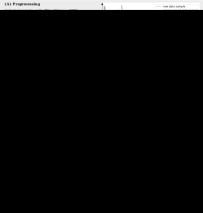
\includegraphics[width=1\textwidth]{img/remodnav_algorithm.pdf}
  \caption{\remodnav workflow. Optional steps and configurable parameters are in bold.}
  \label{fig:alg}
\end{figure*}


\subsection*{Preprocessing}

The goal of data preprocessing is to compute a time series of eye movement
velocities on which the event detection algorithm can be executed, while jointly
reducing non-movement-related noise in the data as much as possible. 

First, implausible spikes in the coordinate time series are removed with a
heuristic spike filter \citep{stampe1993} (\fig{alg}A, 1). This filter is
standard in many eye tracking toolboxes and often used for preprocessing
\citep[\eg][]{Nystrom2010AnData}.
%
Data samples around signal loss (\eg eye blinks) can be nulled in order to
remove spurious movement signals (\param{dilate\_nan},
\param{min\_blink\_duration}; \fig{alg}A, 2).
%
Coordinate time series are temporally filtered in two different ways
(\fig{alg}A, 3). A relatively large median filter (\param{median\_
filter\_length}) is used to emphasize long-distance saccades.  This type of
filtered data is later used for a coarse segmentation of a time series into
shorter intervals between major saccades.
%
Separately, data are also smoothed with a Savitzky-Golay filter
(\param{savgol\_ \{length,polyord\}}). All event detection beyond the
localization of major saccades for time series chunking is performed on this
type of filtered data.

After spike-removal and temporal filtering, movement velocities and
accelerations are computed (\fig{alg}A, 4-5). To
disregard biologically implausible measurements, a configurable maximum
velocity (\param{max\_vel}) is enforced---samples exceeding this threshold
are replaced by this set value.

\begin{table*}[tbp]
  \caption{Algorithm parameters and their default values}
  \label{tab:parameters}
  \small
  \begin{tabular}{lp{85mm}l}
    \textbf{Name} & \textbf{Description} & \textbf{Value} \\
    & & \\
    \multicolumn{3}{l}{\textit{Preprocessing (in order of application during processing)}} \\
    \texttt{px2deg} &
    size of a single (square) pixel in degrees of visual angle &
    no default [\unit{deg/s}]\\
    \texttt{sampling\_rate} &
    temporal data sampling rate/frequency &
    no default [\unit{Hz}]\\
    \texttt{min\_blink\_duration} &
    missing data windows shorter than this duration will not be considered for \texttt{dilate\_nan}&
    \unit[0.02]{s}\\
    \texttt{dilate\_nan} &
    duration for which to replace data by missing data markers on either side of a
    signal-loss window &
    \unit[0.01]{s}\\
    \texttt{median\_filter\_length} &
    smoothing median-filter size (for initial data chunking only) &
    \unit[0.05]{s}\\
    \texttt{savgol\_length} &
    size of Savitzky-Golay filter for noise reduction&
    \unit[0.019]{s}\\
    \texttt{savgol\_polyord} &
    polynomial order of Savitzky-Golay filter for noise reduction&
    2\\
    \texttt{max\_vel} &
    maximum velocity threshold, will replace value with maximum, and issue
    warning if exceeded to inform about
    potentially inappropriate filter settings
    (default value based on \cite{holmqvist2011eye})&
    \unit[1000]{deg/s}\\

    \\\multicolumn{3}{l}{\textit{Event detection}} \\
    \texttt{min\_saccade\_duration} &
    minimum duration of a saccade event candidate &
    \unit[0.01]{s}\\
    \texttt{max\_pso\_duration} &
    maximum duration of a post-saccadic oscillation (glissade) candidate &
    \unit[0.04]{s}\\
    \texttt{min\_fixation\_duration} &
    minimum duration of a fixation event candidate &
    \unit[0.04]{s}\\
    \texttt{min\_pursuit\_duration} &
    minimum duration of a pursuit event candidate &
    \unit[0.04]{s}\\
    \texttt{min\_intersaccade\_duration} &
    no saccade detection is performed in windows shorter than twice this value, plus minimum saccade and PSO duration&
    \unit[0.04]{s}\\
    \texttt{noise\_factor} &
    adaptive saccade onset threshold velocity is the median absolute deviation of velocities in the window of interest, times this factor (peak velocity threshold is twice the onset velocity); increase for noisy data to reduce false positives \citep[equivalent: 3.0]{Nystrom2010AnData}&
    5\\
    \texttt{velthresh\_startvelocity} &
    start value for adaptive velocity threshold algorithm \citep{Nystrom2010AnData}, should
    be larger than any conceivable minimum saccade velocity &
    \unit[300]{deg/s}\\
    \texttt{max\_initial\_saccade\_freq} &
    maximum saccade frequency for initial detection of major saccades, initial data
    chunking is stopped if this frequency is reached (should be smaller than an expected
    (natural) saccade frequency in a particular context), default based on literature reports of a natural, free-viewing saccade frequency of \unit[$\sim$1.7 $\pm$0.3]{Hz} during a movie stimulus \citep{amit2017temporal} &
    \unit[2]{Hz}\\
    \texttt{saccade\_context\_window\_length} &
    size of a window centered on any velocity peak for adaptive determination of
    saccade velocity thresholds (for initial data chunking only) &
    \unit[1]{s}\\
    \texttt{lowpass\_cutoff\_freq} &
    cut-off frequency of a Butterworth low-pass filter applied to determine drift
    velocities in a pursuit event candidate &
    \unit[4]{Hz}\\
    \texttt{pursuit\_velthresh} &
    fixed drift velocity threshold to distinguish periods of pursuit from periods of fixation; higher than natural ocular drift velocities during fixations (e.g. \cite{GOLTZ1997789}; \cite{cherici2012}) &
    \unit[2]{deg/s}\\
  \end{tabular}
\end{table*}



\subsection*{Event detection}

\subsubsection*{Saccade velocity threshold}

Except for a few modifications, \remodnav\ employs the adaptive saccade
detection algorithm proposed by \cite{Nystrom2010AnData}, where saccades are
initially located by thresholding the velocity time series by a critical value.
Starting from an initial velocity threshold (\param{velthresh\_startvelocity},
termed $PT_1$ in NH), the critical value is determined adaptively by computing
the variance of sub-threshold velocities ($V$), and placing the new velocity
threshold at:
%
\begin{equation} PT_n = \overline{V}_{n-1} + F \times \sqrt{{\sum(V_{n-1} -
  \overline{V}_{n-1})^2} \over {N-1}} \end{equation}
%
where $F$ determines how many standard deviations above the average velocity
the new threshold is located.  This procedure is repeated until it stabilizes
on a threshold velocity.
%
\begin{equation} |PT_n - PT_{n-1}| < 1^\circ/sec \end{equation}

\remodnav\ alters this algorithm by using robust statistics that are more
suitable for the non-normal distribution of velocities \citep{Friedman2018},
such that the new threshold is computed by:
%
\begin{equation}\label{eq:threshold}
PT_n = median({V}_{n-1}) + F \times MAD({V}_{n-1})
\end{equation}
%
where $MAD$ is the median absolute deviation, and $F$ is a
scalar parameter of the algorithm.

\subsection*{Time series chunking}

As the algorithm aims to be applicable to prolonged recordings without an
inherent trial structure and inhomogeneous noise levels, the time series needs
to be split into shorter chunks to prevent the negative impact of sporadic
noise flares on the aforementioned adaptive velocity thresholding procedure.

\remodnav\ implements this chunking by determining a critical velocity on a
median-filtered (\param{median\_ filter\_length}) time series comprising the
full duration of a recording (\fig{alg}D). Due to potentially elevated noise
levels, the resulting threshold tends to overestimate an optimal threshold.
Consequently, only periods of fastest eye movements will exceed this threshold.
All such periods of consecutive above-threshold velocities are weighted by the
sum of these velocities. Boundaries of time series chunks are determined by
selecting such events sequentially (starting with the largest sums), until a
maximum average frequency across the whole time series is reached
(\param{max\_initial\_saccade\_ freq}). The resulting chunks represent data
intervals between saccades of maximum magnitude in the respective data.


\subsection*{Detection of saccades and post-saccadic oscillations}

Detection of these event types is identical to the NH algorithm, only the data
context and metrics for determining the velocity thresholds differ.  For
saccades that also represent time series chunk boundaries (event label
\texttt{SACC}), a context of \unit[1]{s}
(\param{saccade\_context\_window\_ length}) centered on the peak velocity is
used by default, for any other saccade (event label \texttt{ISAC}) the entire
time series chunk represents that context (\fig{alg}E).

Peak velocity threshold and on/offset velocity threshold are then determined by
equation \ref{eq:threshold} with $F$ set to $2\times\mathtt{noise\_factor}$ and
\param{noise\_factor}, respectively. Starting from a velocity peak, the
immediately preceding and the following velocity minima that do not exceed the
on/offset threshold are located and used as event boundaries. Qualifying events
are rejected if they do not exceed a configurable minimum duration or violate
the set saccade maximum proximity criterion (\param{min\_ saccade\_duration},
\param{min\_intersaccade\_duration}).

As in NH, post-saccadic oscillations are events that immediately follow a
saccade, where the velocity exceeds the saccade velocity threshold within a short
time window (\param{max\_pso\_duration}). \remodnav\ distinguishes low-velocity
(event label \texttt{LPSO} for chunk boundary event, \texttt{ILPS} otherwise)
and high-velocity oscillations (event label \texttt{HPSO} or \texttt{IHPS}),
where the velocity exceeds the saccade onset or peak velocity threshold,
respectively.

\subsection*{Pursuit and fixation detection}

For all remaining, unlabeled time series segments that are longer than a
minimum duration (\param{min\_fixation\_ duration}), velocities are low-pass
filtered (Butterworth, \param{lowpass\_cutoff\_freq}). Any segments
exceeding a minimum velocity threshold (\param{pursuit\_velthresh})\todo{re-find citation for default value} are
classified as pursuit (event label \texttt{PURS}). Pursuit on/offset detection
uses the same approach as that for saccades: search for local minima preceding
and following the above threshold velocities.
%
Any remaining segment that does not qualify as a pursuit event is classified
as a fixation (event label \texttt{FIXA}).


\subsection*{Operation}\label{op}

\remodnav\ is free and open-source software, written in the Python language and
released under the terms of the MIT license. In addition to the Python standard
library it requires the Python packages
%
NumPy \citep{oliphant2006guide},
Matplotlib \citep{hunter2007matplotlib},
statsmodels \citep{seabold2010statsmodels},
and SciPy \citep{JOP+2001} as software dependencies.
Furthermore, DataLad \citep{HH+2013},
and Pandas \citep{mckinney2010data}
%
have to be available to run the test
battery. \remodnav\ itself, and all software dependencies are available on all
major operating systems.  There are no particular hardware requirements for
running the software other than sufficient memory to load and process the data.

A typical program invocation looks like
%
\begin{verbatim}
remodnav <inputfile> <outputfile> \
    <px2deg> <samplingrate>
\end{verbatim}
%
where \texttt{<inputfile>} is the name of a tab-separated-value (TSV) text file
with one gaze coordinate sample per line. An input file can have any number of
columns, only the first two columns are read and interpreted as $X$ and $Y$
coordinates. The second argument \texttt{<outputfile>} is the file name of a
BIDS-compliant \citep{gorgolewski2016brain} TSV text file that will contain a
report on one detected eye movement event per line, with onset and offset time,
onset and offset coordinates, amplitude, peak velocity, median velocity and
average velocity. The remaining arguments are the only two mandatory
parameters: the conversion factor from pixels to visual degrees, \ie the visual
angle of a single (square) pixel (\texttt{<px2deg>} in \unit{deg/s}), and the
temporal sampling rate (\texttt{<sampling\_rate>} in \unit{Hz}).

All additionally supported parameters (sorted by algorithm step) with their
description and default value, are listed in \tab{parameters}.
While the minimum user input is kept minimal, the number of configurable
parameters is purposefully large to facilitate optimal parameterization for
data with specific properties. Besides the list of detected events, a
visualization of the detection results, together with a time course of
horizontal and vertical gaze position, and velocities is provided for
illustration and initial quality assessment of algorithm performance on each
input data file (see \fig{remodnav} for an example).


\section*{Validation analyses}\label{ana}

% \todo[inline]{three major types of comparison: with andersson human labeling,
% stats of forrest lab recording with andersson video data stats, forrest lab
% vs forrest mri stats. the goal is to show that we are similar to humans, as
% good (or better) as other algorithms (by comparison with scores in
% andersson2017), and proceduce "similar" results on a different movie dataset,
% and similar results across two different qualities of recordings with the
% same stimulus (lab vs MRI). No more, no less IMHO. This all translates to
% three use cases: trial-by-trial data (from anderson), good movie data without
% trial structure (forrest lab), bad movie data (forrest mri)}

% THIS SECTION  WILL BASICALLY SHOW THE INPUTS AND THE OUTPUTS(RESULTS
% BASICALLY)

The selection of datasets and analyses for validating algorithm performance was
guided by three objectives: 1) compare to other existing
solutions; 2) demonstrate plausible results on data from prolonged gaze
coordinate recordings during natural viewing; and 3) illustrate result
robustness on lower-quality data. The following three sections each introduce a
dataset and present the validation results for these objectives.  All analysis
presented here are performed using default parameters (\tab{parameters}), with
no dataset-specific tuning other than the built-in adaptive procedures.


\subsection*{Algorithm comparison}\label{ana_1}

Presently, \cite{Andersson2017} represents the most comprehensive comparative
study on eye movement detection algorithms. Moreover, the dataset employed
in that study was made publicly available. Consequently, evaluating \remodnav\
performance on these data and using their metrics offers a straightforward
approach to relate this new development to alternative solutions.

% dataset
The dataset provided by
\cite{Andersson2017}\footnote{github.com/richardandersson/EyeMovementDetector\linebreak[0]Evaluation}
consists of monocular eye gaze data produced from viewing stimuli from three
distinct categories---images, moving dots and videos. The data release contains
gaze coordinate time series (\unit[500]{Hz} sampling rate), and metadata on
stimulus size and viewing distance.  Importantly, each time point was manually
classified by two expert human raters as one of six event categories: fixation,
saccade, PSO, smooth pursuit, blink and undefined (a sample that did not fit
any other category). A minor labeling mistake reported in \cite{Zemblys2018}
was fixed prior to this validation analysis.

For each stimulus category, we computed the proportion of misclassifications
per event type, comparing \remodnav\ to each of the human coders, and, as a
baseline measure, the human coders against each other.
%
A time point was counted as misclassified if the two compared classifications
did not assign the same label. We limited this analysis to all time points that
were labeled as fixation, saccade, PSO, or pursuit by any method, hence
ignoring the rarely used NaN/blinks or ``undefined" category. For a direct
comparison with the results in \cite{Andersson2017}, the analysis was repeated
while also excluding samples labeled as pursuit. \tab{mclf} shows the
misclassification rates for all pairwise comparisons, in all stimulus types.
In comparison to the NH algorithm, after which the proposed work was modelled,
\remodnav performed consistently better (32/93/70\% average misclassification
vs. \imgMNALMclfWOP/\dotsRAALMclfWOP/ \videoRAALMclfWOP\% worst
misclassification for images, dots, and videos).  Compared to all ten
algorithms evaluated in \citet{Andersson2017}, \remodnav\ exhibits the lowest
misclassification rates across all stimulus categories.
%
When taking smooth pursuit events into account, the misclassification rate
naturally increases, but remains comparably low, and still exceeds the
performance of all algorithms tested in \citet{Andersson2017}.

\begin{table}[tbp]
  % table caption is above the table
  \caption{Proportion of samples in each stimulus category classified in
  disagreement between human coders (MN, RA) and the \remodnav\ algorithm
  (AL). The MC (misclassification) column lists proportions considering
  all four event categories (fixation, saccade, PSO, pursuit), while
  the w/oP (without pursuit) column excludes pursuit events for a direct
  comparison with \citet[][Table 8-10]{Andersson2017}.
  The remaining columns show the percentage of labels assigned to incongruent
  time points by each rater (deviation of their sum from 100\% is due to
  rounding).
  }
  \label{tab:mclf}       % Give a unique label
  % For LaTeX tables use
  \begin{tabular}{llllllll}
    \textbf{Images}&&&&&&&\\
    \hline\noalign{\smallskip}
    Comp & MC & w/oP & Coder & Fix & Sac & PSO & SP \\
    \noalign{\smallskip}\hline\noalign{\smallskip}
    MN-RA & \imgMNRAMCLF & \imgMNRAMclfWOP & MN & \imgMNRAFIXref & \imgMNRASACref & \imgMNRAPSOref & \imgMNRASPref  \\
    --- & --- & --- & RA & \imgMNRAFIXcod & \imgMNRASACcod & \imgMNRAPSOcod & \imgMNRASPcod \\
    MN-AL & \imgMNALMCLF & \imgMNALMclfWOP & MN & \imgMNALFIXref & \imgMNALSACref & \imgMNALPSOref & \imgMNALSPref \\
    --- & --- & --- & AL & \imgMNALFIXcod & \imgMNALSACcod & \imgMNALPSOcod & \imgMNALSPcod \\
    RA-AL & \imgRAALMCLF & \imgRAALMclfWOP & RA & \imgRAALFIXref & \imgRAALSACref & \imgRAALPSOref & \imgRAALSPref \\
    ---& ---& ---& AL & \imgRAALFIXcod & \imgRAALSACcod & \imgRAALPSOcod & \imgRAALSPcod \\
    \noalign{\smallskip}
    \textbf{Dots}&&&&&&&\\
    \hline\noalign{\smallskip}
    Comp & MC & w/oP & Coder & Fix & Sac & PSO & SP \\
    \noalign{\smallskip}\hline\noalign{\smallskip}
    MN-RA & \dotsMNRAMCLF & \dotsMNRAMclfWOP & MN & \dotsMNRAFIXref & \dotsMNRASACref & \dotsMNRAPSOref & \dotsMNRASPref  \\
    --- & --- & --- & RA & \dotsMNRAFIXcod & \dotsMNRASACcod & \dotsMNRAPSOcod & \dotsMNRASPcod \\
    MN-AL & \dotsMNALMCLF & \dotsMNALMclfWOP & MN & \dotsMNALFIXref & \dotsMNALSACref & \dotsMNALPSOref & \dotsMNALSPref \\
    --- & --- & --- & AL & \dotsMNALFIXcod & \dotsMNALSACcod & \dotsMNALPSOcod & \dotsMNALSPcod\\
    RA-AL & \dotsRAALMCLF & \dotsRAALMclfWOP & RA & \dotsRAALFIXref & \dotsRAALSACref & \dotsRAALPSOref & \dotsRAALSPref \\
    ---& ---& ---& AL & \dotsRAALFIXcod & \dotsRAALSACcod & \dotsRAALPSOcod & \dotsRAALSPcod \\
    \noalign{\smallskip}
    \textbf{Videos}&&&&&&&\\
    \hline\noalign{\smallskip}
    Comp & MC & w/oP & Coder & Fix & Sac & PSO & SP \\
    \noalign{\smallskip}\hline\noalign{\smallskip}
    MN-RA & \videoMNRAMCLF & \videoMNRAMclfWOP & MN & \videoMNRAFIXref & \videoMNRASACref & \videoMNRAPSOref & \videoMNRASPref \\
    --- & --- & --- & RA & \videoMNRAFIXcod & \videoMNRASACcod & \videoMNRAPSOcod & \videoMNRASPcod \\
    MN-AL & \videoMNALMCLF & \videoMNALMclfWOP & MN & \videoMNALFIXref & \videoMNALSACref & \videoMNALPSOref & \videoMNALSPref \\
    --- & --- & --- & AL & \videoMNALFIXcod & \videoMNALSACcod & \videoMNALPSOcod & \videoMNALSPcod\\
    RA-AL & \videoRAALMCLF & \videoRAALMclfWOP & RA & \videoRAALFIXref & \videoRAALSACref & \videoRAALPSOref & \videoRAALSPref \\
    ---& ---& ---& AL & \videoRAALFIXcod & \videoRAALSACcod & \videoRAALPSOcod & \videoRAALSPcod \\
    \noalign{\smallskip}\hline
  \end{tabular}
\end{table}

\fig{conf} shows confusion patterns for a comparison of algorithm
classifications with human labeling. While \remodnav\ does not achieve a
labeling similarity that reaches the human inter-rater agreement, it still
performs well. In particular, the relative magnitude of agreement with each
individual human coder for fixations, saccades, and PSOs, resembles the
agreement between the human coders. Classification of smooth
pursuits is consistent with human labels for the categories moving dots, and
videos. However, there is a substantial confusion of fixation and pursuit for
the static images. In a real-world application of \remodnav, pursuit detection
could be disabled (by setting a high pursuit velocity threshold) for data from
static images, if the occurrence of pursuit events can be ruled out a priori.
For this evaluation, however, no such intervention was made.

\begin{figure*}
  % Use the relevant command to insert your figure file.
  % For example, with the graphicx package use
  % TODO make final figure and switch
  %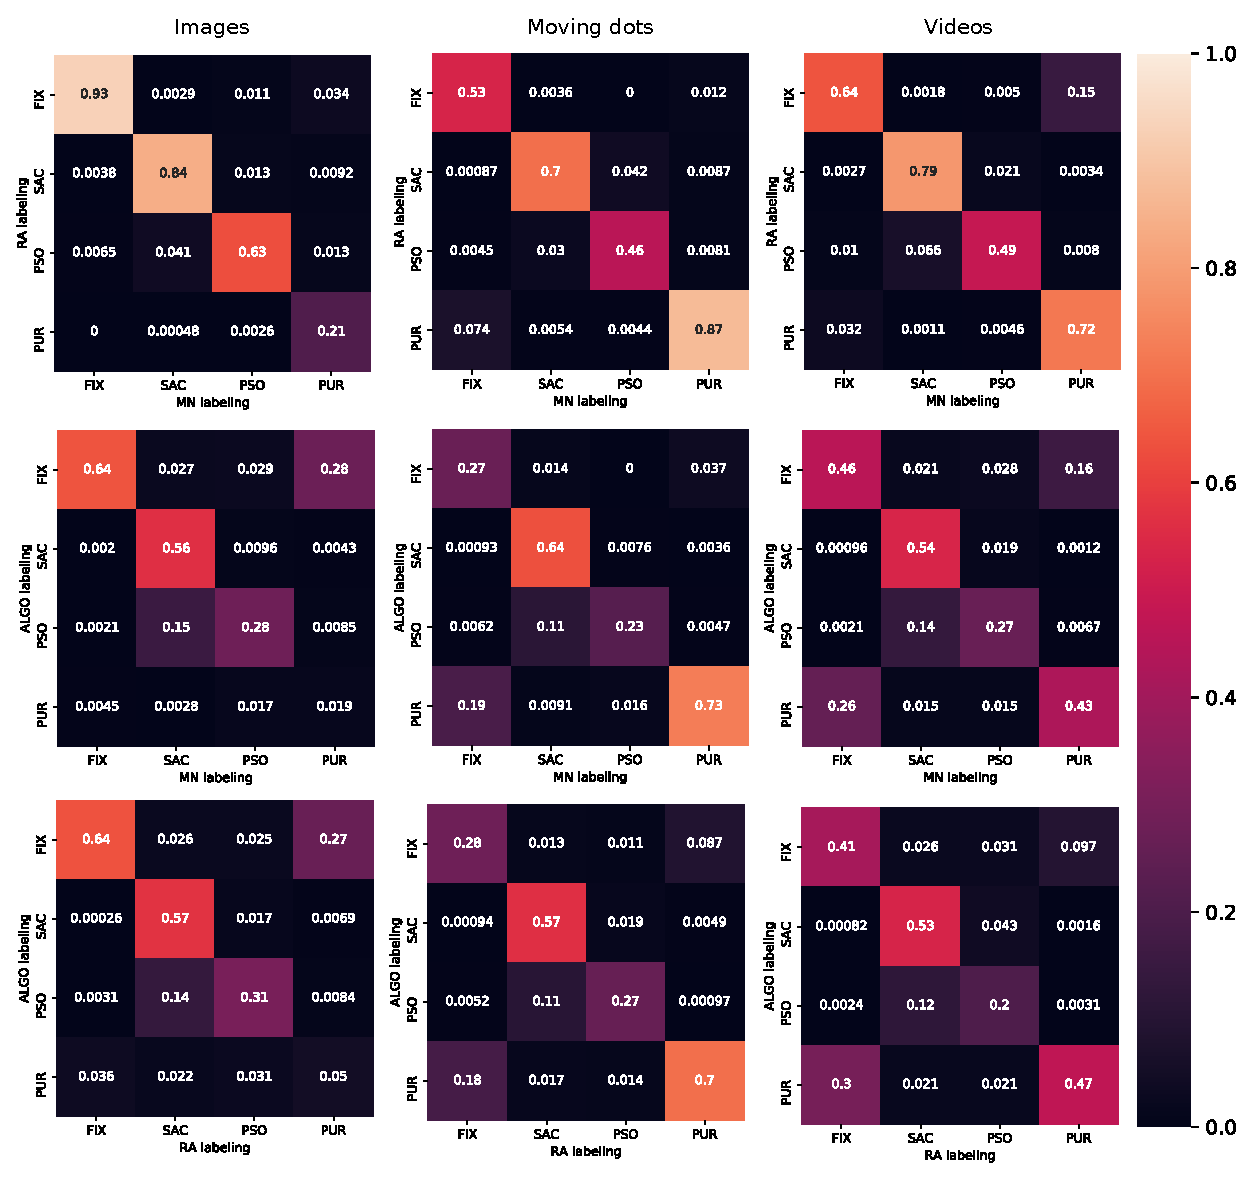
\includegraphics[width=1\textwidth]{img/conf_drawing.eps}
  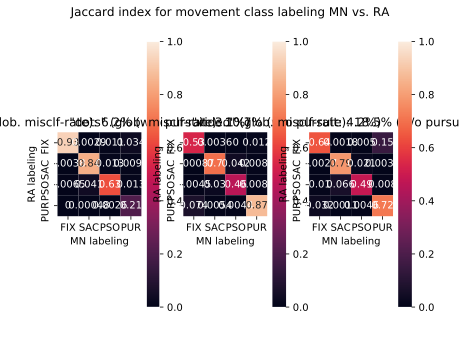
\includegraphics[trim=0 0 0 0,clip,width=1\textwidth]{img/confusion_MN_RA.pdf} \\
  \includegraphics[trim=0 0 0 6mm,clip,width=1\textwidth]{img/confusion_MN_AL.pdf} \\
  \includegraphics[trim=0 0 0 6mm,clip,width=1\textwidth]{img/confusion_RA_AL.pdf}
  % figure caption is below the figure

  \caption{Confusion patterns for pairwise eye movement classification
    comparison of both human raters \citep[MN and RA; ][]{Andersson2017} and the
    \remodnav\ algorithm (AL) for gaze recordings from stimulation with static
    images (left column), moving dots (middle column), and video clips (right
    column).  All matrices present gaze sample based Jaccard indices \citep[JI;
    ][]{jaccard1901etude}. Consequently, the diagonals depict the fraction of
    time points labeled congruently by both raters in relation to the number of
    timepoints assigned to a particular event category by any rater.}
  % Give a unique label
  \label{fig:conf}
\end{figure*}


In order to further rank the performance of the proposed algorithm with respect
to the ten algorithms studied in \citet{Andersson2017}, we followed their
approach to compute root mean square deviations (RMSD) from human labels for
event duration distribution characteristics (mean and standard deviation of
durations, plus number of events) for each stimulus category (images, dots,
videos) and event type (fixations, saccades, PSOs, pursuits). This measure
represents a scalar distribution dissimilarity score that can be used as an
additional comparison metric of algorithm performance that focuses on overall
number and durations of detected events, instead of sample-by-sample
misclassification. The RMSD measure has a lower bound of $0.0$ (identical to
the average of both human raters), with higher values indicating larger
differences \citep[for detail information on the calculation of this metric
see][]{Andersson2017}.

Tables \ref{tab:rmsd_fix}-\ref{tab:rmsd_pur} reproduce \citet[Tables
3-6]{Andersson2017}, and the RMSD calculation for the added rows on \remodnav\
is based on the scores for the human raters given in these original tables. As
acknowledged by the authors, the absolute value of the RMSD scores is not
informative due to scaling with respect to the respective maximum value of each
characteristic.  Therefore, we converted RSMDs for each algorithm and event
type into zero-based ranks (lower is more human-like).

The LNS algorithm \citep{Larsson2013} was found to have the most human-like
performance for saccade and PSO detection in \cite{Andersson2017}.  \remodnav\
performs comparable to LNS for both event types (saccades: $2.0$ vs. $3.3$;
PSOs: $2.3$ vs. $2.0$, mean rank across stimulus categories for LNS and \remodnav,
respectively).

Depending on the stimulus type, different algorithms performed best for
fixation detection. NH performed best for images and videos, but worst for
moving dots. \remodnav\ outperforms all other algorithms in the dots category,
and achieves rank 5 and 6 (middle range) for videos and images, respectively.
Across all stimulus and event categories, \remodnav\ achieves a \todo{why
median now, and mean before}median ranking of $3.0$.

\begin{table*}[p]
  % table caption is above the table
  \caption{RMSD ranks of fixation parameters for various stimulation types}
  \label{tab:rmsd_fix}       % Give a unique label
  % For LaTeX tables use
  \begin{small}
  \begin{tabular*}{\textwidth}{c @{\extracolsep{\fill}}lllllllllllll}
    \hline\noalign{\smallskip}
    & \multicolumn{4}{l}{Images} & \multicolumn{4}{l}{Dots} & \multicolumn{4}{l}{Videos}\\
    Algorithm & Mean & SD & \# & rank &  Mean & SD & \# & rank & Mean & SD & \# & rank \\
    \noalign{\smallskip}\hline\noalign{\smallskip}
    MN        & \FIXimgmnMN   & \FIXimgsdMN   & \FIXimgnoMN   & \rankFIXimgMN   &  \FIXdotsmnMN   & \FIXdotssdMN   & \FIXdotsnoMN   & \rankFIXdotsMN    & \FIXvideomnMN   & \FIXvideosdMN   & \FIXvideonoMN   & \rankFIXvideoMN    \\
    RA        & \FIXimgmnRA   & \FIXimgsdRA   & \FIXimgnoRA   & \rankFIXimgRA   &  \FIXdotsmnRA   & \FIXdotssdRA   & \FIXdotsnoRA   & \rankFIXdotsRA    & \FIXvideomnRA   & \FIXvideosdRA   & \FIXvideonoRA   & \rankFIXvideoRA    \\
    CDT       & \FIXimgmnCDT  & \FIXimgsdCDT  & \FIXimgnoCDT  & \rankFIXimgCDT  &  \FIXdotsmnCDT  & \FIXdotssdCDT  & \FIXdotsnoCDT  & \rankFIXdotsCDT   & \FIXvideomnCDT  & \FIXvideosdCDT  & \FIXvideonoCDT  & \rankFIXvideoCDT   \\
    EM        & -             & -             & -             & -               &  -              & -              & -              & -                 & -               & -               & -               & -                  \\
    IDT       & \FIXimgmnIDT  & \FIXimgsdIDT  & \FIXimgnoIDT  & \rankFIXimgIDT  &  \FIXdotsmnIDT  & \FIXdotssdIDT  & \FIXdotsnoIDT  & \rankFIXdotsIDT   & \FIXvideomnIDT  & \FIXvideosdIDT  & \FIXvideonoIDT  & \rankFIXvideoIDT   \\
    IKF       & \FIXimgmnIKF  & \FIXimgsdIKF  & \FIXimgnoIKF  & \rankFIXimgIKF  &  \FIXdotsmnIKF  & \FIXdotssdIKF  & \FIXdotsnoIKF  & \rankFIXdotsIKF   & \FIXvideomnIKF  & \FIXvideosdIKF  & \FIXvideonoIKF  & \rankFIXvideoIKF   \\
    IMST      & \FIXimgmnIMST & \FIXimgsdIMST & \FIXimgnoIMST & \rankFIXimgIMST &  \FIXdotsmnIMST & \FIXdotssdIMST & \FIXdotsnoIMST & \rankFIXdotsIMST  & \FIXvideomnIMST & \FIXvideosdIMST & \FIXvideonoIMST & \rankFIXvideoIMST  \\
    IHMM      & \FIXimgmnIHMM & \FIXimgsdIHMM & \FIXimgnoIHMM & \rankFIXimgIHMM &  \FIXdotsmnIHMM & \FIXdotssdIHMM & \FIXdotsnoIHMM & \rankFIXdotsIHMM  & \FIXvideomnIHMM & \FIXvideosdIHMM & \FIXvideonoIHMM & \rankFIXvideoIHMM  \\
    IVT       & \FIXimgmnIVT  & \FIXimgsdIVT  & \FIXimgnoIVT  & \rankFIXimgIVT  &  \FIXdotsmnIVT  & \FIXdotssdIVT  & \FIXdotsnoIVT  & \rankFIXdotsIVT   & \FIXvideomnIVT  & \FIXvideosdIVT  & \FIXvideonoIVT  & \rankFIXvideoIVT   \\
    NH        & \FIXimgmnNH   & \FIXimgsdNH   & \FIXimgnoNH   & \rankFIXimgNH   &  \FIXdotsmnNH   & \FIXdotssdNH   & \FIXdotsnoNH   & \rankFIXdotsNH    & \FIXvideomnNH   & \FIXvideosdNH   & \FIXvideonoNH   & \rankFIXvideoNH    \\
    BIT       & \FIXimgmnBIT  & \FIXimgsdBIT  & \FIXimgnoBIT  & \rankFIXimgBIT  &  \FIXdotsmnBIT  & \FIXdotssdBIT  & \FIXdotsnoBIT  & \rankFIXdotsBIT   & \FIXvideomnBIT  & \FIXvideosdBIT  & \FIXvideonoBIT  & \rankFIXvideoBIT   \\
    LNS       & -             & -             & -             &  -              &  -              & -              & -              &  -                & -               & -               & -               &  -                 \\
    \remodnav\ & \FIXimgmnRE   & \FIXimgsdRE   & \FIXimgnoRE   & \rankFIXimgRE   &  \FIXdotsmnRE   & \FIXdotssdRE   & \FIXdotsnoRE   & \rankFIXdotsRE    & \FIXvideomnRE   & \FIXvideosdRE   & \FIXvideonoRE   & \rankFIXvideoRE    \\
    \noalign{\smallskip}\hline
  \end{tabular*}
  \end{small}

  \textit{Note}: Fixation distribution parameters for the algorithms
  reported in \citet{Andersson2017} and \remodnav\ (bottom row). RMSDs
  were converted into ranks (lower is better).

\end{table*}

\begin{table*}[p]
  % table caption is above the table
  \caption{RMSD ranks of saccade parameters for various stimulation types}
  \label{tab:rmsd_sac}       % Give a unique label
  % For LaTeX tables use
  \begin{small}
  \begin{tabular*}{\textwidth}{c @{\extracolsep{\fill}}lllllllllllll}
    \hline\noalign{\smallskip}
    & \multicolumn{4}{l}{Images} & \multicolumn{4}{l}{Dots} & \multicolumn{4}{l}{Videos}\\
    Algorithm & Mean & SD & \# & rank &  Mean & SD & \# & rank & Mean & SD & \# & rank \\
    \noalign{\smallskip}\hline\noalign{\smallskip}
    MN        & \SACimgmnMN   & \SACimgsdMN   & \SACimgnoMN   & \rankSACimgMN   &  \SACdotsmnMN   & \SACdotssdMN   & \SACdotsnoMN   & \rankSACdotsMN    & \SACvideomnMN   & \SACvideosdMN   & \SACvideonoMN   & \rankSACvideoMN    \\
    RA        & \SACimgmnRA   & \SACimgsdRA   & \SACimgnoRA   & \rankSACimgRA   &  \SACdotsmnRA   & \SACdotssdRA   & \SACdotsnoRA   & \rankSACdotsRA    & \SACvideomnRA   & \SACvideosdRA   & \SACvideonoRA   & \rankSACvideoRA    \\
    CDT       & -             & -             & -             & -               &  -              & -              & -              & -                 & -               & -               & -               & -                  \\
    EM        & \SACimgmnEM   & \SACimgsdEM   & \SACimgnoEM   & \rankSACimgEM    &  \SACdotsmnEM   & \SACdotssdEM   & \SACdotsnoEM   & \rankSACdotsEM    & \SACvideomnEM   & \SACvideosdEM   & \SACvideonoEM   & \rankSACvideoEM    \\
    IDT       & \SACimgmnIDT  & \SACimgsdIDT  & \SACimgnoIDT  & \rankSACimgIDT  &  \SACdotsmnIDT  & \SACdotssdIDT  & \SACdotsnoIDT  & \rankSACdotsIDT   & \SACvideomnIDT  & \SACvideosdIDT  & \SACvideonoIDT  & \rankSACvideoIDT   \\
    IKF       & \SACimgmnIKF  & \SACimgsdIKF  & \SACimgnoIKF  & \rankSACimgIKF  &  \SACdotsmnIKF  & \SACdotssdIKF  & \SACdotsnoIKF  & \rankSACdotsIKF   & \SACvideomnIKF  & \SACvideosdIKF  & \SACvideonoIKF  & \rankSACvideoIKF   \\
    IMST      & \SACimgmnIMST & \SACimgsdIMST & \SACimgnoIMST & \rankSACimgIMST &  \SACdotsmnIMST & \SACdotssdIMST & \SACdotsnoIMST & \rankSACdotsIMST  & \SACvideomnIMST & \SACvideosdIMST & \SACvideonoIMST & \rankSACvideoIMST  \\
    IHMM      & \SACimgmnIHMM & \SACimgsdIHMM & \SACimgnoIHMM & \rankSACimgIHMM &  \SACdotsmnIHMM & \SACdotssdIHMM & \SACdotsnoIHMM & \rankSACdotsIHMM  & \SACvideomnIHMM & \SACvideosdIHMM & \SACvideonoIHMM & \rankSACvideoIHMM  \\
    IVT       & \SACimgmnIVT  & \SACimgsdIVT  & \SACimgnoIVT  & \rankSACimgIVT  &  \SACdotsmnIVT  & \SACdotssdIVT  & \SACdotsnoIVT  & \rankSACdotsIVT   & \SACvideomnIVT  & \SACvideosdIVT  & \SACvideonoIVT  & \rankSACvideoIVT   \\
    NH        & \SACimgmnNH   & \SACimgsdNH   & \SACimgnoNH   & \rankSACimgNH   &  \SACdotsmnNH   & \SACdotssdNH   & \SACdotsnoNH   & \rankSACdotsNH    & \SACvideomnNH   & \SACvideosdNH   & \SACvideonoNH   & \rankSACvideoNH    \\
    BIT       & -             & -             & -             & -               &  -              & -              & -              & -                 & -               & -               & -               & -                  \\
    LNS       & \SACimgmnLNS  & \SACimgsdLNS  & \SACimgnoLNS  & \rankSACimgLNS  &  \SACdotsmnLNS  & \SACdotssdLNS  & \SACdotsnoLNS  & \rankSACdotsLNS   & \SACvideomnLNS  & \SACvideosdLNS  & \SACvideonoLNS  & \rankSACvideoLNS   \\
    \remodnav\ & \SACimgmnRE   & \SACimgsdRE   & \SACimgnoRE   & \rankSACimgRE   &  \SACdotsmnRE   & \SACdotssdRE   & \SACdotsnoRE   & \rankSACdotsRE    & \SACvideomnRE   & \SACvideosdRE   & \SACvideonoRE   & \rankSACvideoRE    \\
    \noalign{\smallskip}\hline
  \end{tabular*}
  \end{small}

  \textit{Note}: Saccade distribution parameters for the algorithms
  reported in \citet{Andersson2017} and \remodnav\ (bottom row). RMSDs
  were converted into ranks (lower is better).

\end{table*}

\begin{table*}[p]
  % table caption is above the table
  \caption{RMSD ranks of PSO parameters for various stimulation types}
  \label{tab:rmsd_pso}       % Give a unique label
  % For LaTeX tables use
  \begin{small}
  \begin{tabular*}{\textwidth}{c @{\extracolsep{\fill}}lllllllllllll}
    \hline\noalign{\smallskip}
    & \multicolumn{4}{l}{Images} & \multicolumn{4}{l}{Dots} & \multicolumn{4}{l}{Videos}\\
    Algorithm & Mean & SD & \# & rank &  Mean & SD & \# & rank & Mean & SD & \# & rank \\
    \noalign{\smallskip}\hline\noalign{\smallskip}
    MN        & \PSOimgmnMN   & \PSOimgsdMN   & \PSOimgnoMN   & \rankPSOimgMN   &  \PSOdotsmnMN   & \PSOdotssdMN   & \PSOdotsnoMN   & \rankPSOdotsMN    & \PSOvideomnMN   & \PSOvideosdMN   & \PSOvideonoMN   & \rankPSOvideoMN    \\
    RA        & \PSOimgmnRA   & \PSOimgsdRA   & \PSOimgnoRA   & \rankPSOimgRA   &  \PSOdotsmnRA   & \PSOdotssdRA   & \PSOdotsnoRA   & \rankPSOdotsRA    & \PSOvideomnRA   & \PSOvideosdRA   & \PSOvideonoRA   & \rankPSOvideoRA    \\
    NH        & \PSOimgmnNH   & \PSOimgsdNH   & \PSOimgnoNH   & \rankPSOimgNH   &  \PSOdotsmnNH   & \PSOdotssdNH   & \PSOdotsnoNH   & \rankPSOdotsNH    & \PSOvideomnNH   & \PSOvideosdNH   & \PSOvideonoNH   & \rankPSOvideoNH    \\
    LNS       & \PSOimgmnLNS  & \PSOimgsdLNS  & \PSOimgnoLNS  & \rankPSOimgLNS  &  \PSOdotsmnLNS  & \PSOdotssdLNS  & \PSOdotsnoLNS  & \rankPSOdotsLNS   & \PSOvideomnLNS  & \PSOvideosdLNS  & \PSOvideonoLNS  & \rankPSOvideoLNS   \\
    \remodnav\ & \PSOimgmnRE   & \PSOimgsdRE   & \PSOimgnoRE   & \rankPSOimgRE   &  \PSOdotsmnRE   & \PSOdotssdRE   & \PSOdotsnoRE   & \rankPSOdotsRE    & \PSOvideomnRE   & \PSOvideosdRE   & \PSOvideonoRE   & \rankPSOvideoRE    \\
    \noalign{\smallskip}\hline
  \end{tabular*}
  \end{small}

  \textit{Note}: PSO distribution parameters for the algorithms
  reported in \citet{Andersson2017} and \remodnav\ (bottom row). RMSDs
  were converted into ranks (lower is better).

\end{table*}

\begin{table*}[tbp]
  % table caption is above the table
  \caption{RMSD ranks of pursuit parameters for various stimulation types}
  \label{tab:rmsd_pur}       % Give a unique label
  % For LaTeX tables use
  \begin{small}
  \begin{tabular*}{\textwidth}{c @{\extracolsep{\fill}}lllllllllllll}
    \hline\noalign{\smallskip}
    & \multicolumn{4}{l}{Images} & \multicolumn{4}{l}{Dots} & \multicolumn{4}{l}{Videos}\\
    Algorithm & Mean & SD & \# & rank &  Mean & SD & \# & rank & Mean & SD & \# & rank \\
    \noalign{\smallskip}\hline\noalign{\smallskip}
    MN        & \PURimgmnMN   & \PURimgsdMN   & \PURimgnoMN   & \rankPURimgMN   &  \PURdotsmnMN   & \PURdotssdMN   & \PURdotsnoMN   & \rankPURdotsMN    & \PURvideomnMN   & \PURvideosdMN   & \PURvideonoMN   & \rankPURvideoMN    \\
    RA        & \PURimgmnRA   & \PURimgsdRA   & \PURimgnoRA   & \rankPURimgRA   &  \PURdotsmnRA   & \PURdotssdRA   & \PURdotsnoRA   & \rankPURdotsRA    & \PURvideomnRA   & \PURvideosdRA   & \PURvideonoRA   & \rankPURvideoRA    \\
    \remodnav\ & \PURimgmnRE   & \PURimgsdRE   & \PURimgnoRE   & \rankPURimgRE   &  \PURdotsmnRE   & \PURdotssdRE   & \PURdotsnoRE   & \rankPURdotsRE    & \PURvideomnRE   & \PURvideosdRE   & \PURvideonoRE   & \rankPURvideoRE    \\
    \noalign{\smallskip}\hline
  \end{tabular*}
  \end{small}

  \textit{Note}: Smooth pursuit distribution parameters for the algorithms
  reported in \citet{Andersson2017} and \remodnav\ (bottom row). RMSDs
  were converted into ranks (lower is better).

\end{table*}


Taken together, \remodnav\ yields classification results that are, on average,
more human-like than any other algorithm tested on the dataset and metrics put
forth by \citet{Andersson2017}. In particular, its performance largely equals
or exceeds that of the original NH algorithm. NH outperforms it only for
fixation detection in the image and video category, but in these categories
\remodnav\ also classifies comparatively well. These results are an indication
that the changes to the NH algorithm proposed here to improve upon its
robustness are not detrimental to its performance on data from conventional
paradigms and stimuli.


\subsection*{Prolonged natural viewing}\label{ana_2}

Given that \remodnav\ yielded plausible results for the "video" stimulus
category data in the \citet{Andersson2017} dataset (\fig{conf}, and
Tables~\ref{tab:rmsd_fix}-\ref{tab:rmsd_pur}, right columns), we determined
whether it is capable of analyzing data from dynamic stimulation without a
trial structure.

As a test dataset we used publicly available eye tracking data from the
\textit{studyforrest.org} project, where 15~participants were recorded watching
a feature-length (\unit[$\approx$2]{h}) movie in a laboratory setting
\citep{Hanke2016}. Eye movements were measured by an Eyelink 1000 with a
standard desktop mount (software version 4.51; SR Research Ltd., Mississauga,
Ontario, Canada) and a sampling rate of 1000Hz. The movie stimulus was
presented on a \unit[$522\times294$]{mm} LCD monitor at a resolution of
\unit[$1920\times1280$]{px} at a viewing distance of \unit[85]{cm}. Participants
watched the movie in eight approximately \unit[15]{min} long segments,
with measurement recalibration before every segment.

\begin{figure*}[tbp]
  \includegraphics[trim=0 8mm 3mm 0,clip,width=.5\textwidth]{img/mainseq_lab_300dpi.png}
  \includegraphics[trim=8mm 8mm 0 0,clip,width=.5\textwidth-3.3mm]{img/mainseq_sub_lab_300dpi.png} \\
  \includegraphics[trim=0 0 3mm 0,clip,width=.5\textwidth]{img/mainseq_mri_300dpi.png}
  \includegraphics[trim=8mm 0 0 0,clip,width=.5\textwidth-3.3mm]{img/mainseq_sub_mri_300dpi.png}

  \caption{Main sequence of eye movement events during one 15 minute sequence of
  the movie (segment 2) for lab (top), and MRI participants (bottom). Data
  across all participants per dataset is shown on the left, and data for a single
  exemplary participant on the right.}

  \label{fig:overallComp}
\end{figure*}

As no manual eye movement event labeling exists for these data, algorithm
evaluation was limited to a comparison of marginal distributions and well-known
properties, such as the log-log-linear relationship of saccade amplitude and
saccade peak velocity \citep{bahill1975main}. \fig{overallComp} (top row)
depicts this main sequence relationship.
%
Additionally, \fig{dist} (top row) shows duration histograms for all four event
types across all participants. Shapes and locations of these distributions
match previous reports in the literature, such as a strong bias towards short
(less than \unit[500]{ms}) fixations for dynamic stimuli
\citep[Fig.~3]{dorr2010variability}, peak number of PSOs with durations between
\unit[10-20]{ms} \citep[Fig.~11]{Nystrom2010AnData}, and a non-Gaussian saccade
duration distribution located below \unit[100]{ms} \citep[Fig.~8, albeit for
static scene perception]{Nystrom2010AnData}.

Overall, the presented summary statistics suggest that \remodnav\ is capable
of detecting eye movements with plausible characteristics, in prolonged
gaze recordings without a trial structure. A visualization of such a detection
result is depicted in \fig{remodnav} (top row).

\begin{figure*}
  % Use the relevant command to insert your figure file.
  \includegraphics[width=0.24\textwidth]{img/hist_fixation_lab.pdf}
  \includegraphics[width=0.24\textwidth]{img/hist_saccade_lab.pdf}
  \includegraphics[width=0.24\textwidth]{img/hist_PSO_lab.pdf}
  \includegraphics[width=0.24\textwidth]{img/hist_pursuit_lab.pdf} \\
  \includegraphics[width=0.24\textwidth]{img/hist_fixation_mri.pdf}
  \includegraphics[width=0.24\textwidth]{img/hist_saccade_mri.pdf}
  \includegraphics[width=0.24\textwidth]{img/hist_PSO_mri.pdf}
  \includegraphics[width=0.24\textwidth]{img/hist_pursuit_mri.pdf} \\
  % figure caption is below the figure
  \caption{Comparison of eye movement event duration distributions for the
    high-quality lab sample (top row), and the lower quality MRI sample
    (bottom row) across all participants (each $N=15$), and the entire duration of
    the same feature-length movie stimulus. All histograms depict absolute
    number of events. Visible differences are limited to an overall lower number of
    events, and fewer long saccades for the MRI sample. These are attributable
    to a higher noise level and more signal loss \citep[compare][Fig.
    4b]{Hanke2016} in the MRI sample, and to stimulus size differences
    (\unit[23.75]{\textdegree} MRI vs. \unit[34]{\textdegree} lab).}
  \label{fig:dist}
  % Give a unique label
\end{figure*}

\begin{figure*}[tbp]
  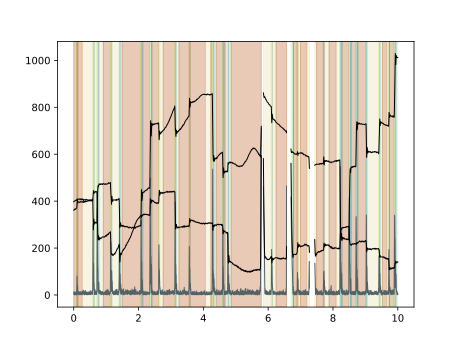
\includegraphics[trim=0 8mm 0 0,clip,width=1\textwidth]{img/remodnav_lab.pdf} \\
  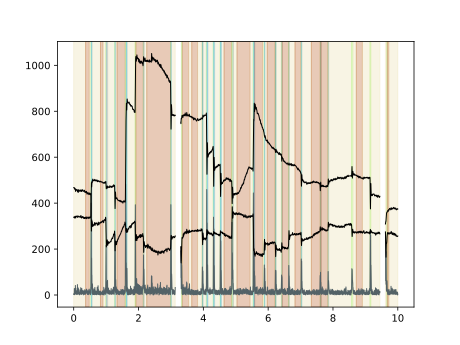
\includegraphics[trim=0 0 0 2mm,clip,width=1\textwidth-1mm]{img/remodnav_mri.pdf}\\
  \caption{Exemplary eye movement detection results for the same \unit[10]{s} excerpt
  of a movie stimulus for a single participant in the high quality lab sample (top),
  and in the lower quality MRI sample (bottom). The plots show filtered gaze coordinates
  (black), computed velocity time series (gray) overlayed on the eye movement event segmentation
  with periods of fixation (green), pursuit (beige), saccades (blue), and
  high/low-velocity post-saccadic oscillations (dark/light purple). The variable noise
  level, and prolonged signal loss (white) visible in the MRI sample represent
  a challenge for algorithms. \remodnav\ uses an adaptive approach that determines major
  saccade events first, and subsequently tunes the velocity threshold to short time
  windows between these events. Figures like this accompany the program output to
  facilitate quality control and discovery of inappropriate preprocessing and detection
  parameterization.}

  \label{fig:remodnav}
\end{figure*}


\subsection*{Lower-quality data}\label{ana_3}

An explicit goal for \remodnav\ development was robust performance on
lower-quality data. While lack of quality cannot be arbitrarily compensated and
will inevitably lead to misses in eye movement detection, it is beneficial for
any further analysis if operation on noisy data does not introduce unexpected
event property biases.

In order to investigate noise-robustness we ran \remodnav\ on another
publicly available dataset from the \textit{studyforrest.org} project, where 15
different participants watched the exact same movie stimulus, but this time
while lying on their back in the bore of an MRI scanner \citep{Hanke2016}.
These data were recorded with a different Eyelink 1000 (software version 4.594)
equipped with an MR-compatible telephoto lens and illumination kit (SR Research
Ltd., Mississauga, Ontario, Canada) at \unit[1000]{Hz} during simultaneous fMRI
acquisition. The movie was presented at a viewing distance of \unit[$63$]{cm}
on a \unit[26]{cm} (\unit[$1280\times1024$]{px}) LCD screen in 720p resolution
at full width, yielding a substantially smaller stimulus size, compared to the
previous stimulation setup. The eye tracking camera was mounted outside the
scanner bore and recorded the participants left eye at a distance of about
\unit[100]{cm}.  Compared to the lab-setup, physical limitations of the scanner
environment, and sub-optimal infrared illumination lead to substantially
noisier data, as evident from a generally higher amount of data loss and a
larger spatial uncertainty \citep[Technical Validation]{Hanke2016}. An example
of the amplified and variable noise pattern is shown in \fig{remodnav} (bottom
row, black lines). Except for the differences in stimulation setup, all other
aspects of data acquisition, eye tracker calibration, and data processing
where identical to the previous dataset.

We performed the identical analysis as before, in order to compare performance
between a high and lower-quality data acquisition.
Figures~\ref{fig:overallComp}-\ref{fig:remodnav} depict the results for the
lab-quality dataset, and the MRI-scanner dataset in the top and bottom rows,
respectively.

% N+H describe: "Data quality is related to accuracy, precision, percentage of
% data loss, perhaps in addition to a subjective rating from the person
% responsible for the recording"

Overall, the detection results exhibit strong similarity, despite the potential
behavioral impact of watching a movie while lying on their back and looking
upwards on the participants, or the well known effect of increasing fatigue
during a two-hour session in an MRI-scanner. In particular, saccade amplitude
and peak velocity exhibit a clear main-sequence relationship that resembles
that found for the lab acquisition (\fig{overallComp}). Duration distributions
for fixations, PSOs, and pursuit are strikingly similar between the two
datasets (\fig{dist}), except for a generally lower number of detected events
for the MRI experiment, which could be explained by the higher noise level and
fraction of signal loss. There is a notable difference regarding the saccade
duration distributions, with a bias towards shorter saccades in the MRI
dataset. This effect may be attributable to the differences in stimulus size
(30\% smaller in the MRI environment).


\section*{Conclusion}\label{con}


Based on the adaptive, velocity-based algorithm for fixation, saccade, and
glissade detection by \cite{Nystrom2010AnData}, we have developed a novel and
robust algorithm for the classification of various eye movements in eye
tracking data from dynamic stimulation.  The combined results from all analyses
are encouraging. Based on data from dynamic and static stimulation from the
Andersson dataset, \remodnav\ performs well and even outperforms contemporary
algorithms---especially in the case of dynamic stimulation. Therefore, we
are confident that \remodnav\ is currently a good choice for event detection
from eye gaze data obtained during dynamic stimulation.  Furthermore, the
algorithm yields similar, and thus robust, results for high and lower quality
data. We specifically developed \remodnav\ to yield robust results with dynamic
stimulation, in particular noisy data such as the eye tracking data recorded
simultaneously with fMRI acquisition. These results confirm that \remodnav\ is
well able to detect eye movements from dynamic stimulation, even when the
quality of data is lower. Therefore, the algorithm is a promising tool for
research paradigms with dynamic stimuli where lower data quality is an inherent
property of the acquisition procedure; such as simultaneous fMRI and eye gaze
recordings, or usage of remote eye trackers.  Furthermore, the algorithm proved
to be well applicable to other types of stimulation. Its classification
performance on static images was good. This demonstrates that our changes to
the original NH algorithm did not interfere with where it performed best. 
Lastly, \remodnav\ is a user-friendly tool with options available to customize
it to individual use cases. It is OS independent, uses only freely available
software, is easily installable, provides simple command-line execution, and is
ready-to-use without manual labeling or other forms of training data being
required. As such, REMoDNaV is a versatile tool that provides researchers with
a robust method to classify eye movements obtained from different types of
stimulation.

Just as \cite{Andersson2017}, we considered human annotations to be a gold
standard in event detection when we compared different algorithms performances.
The implications of the obtained results from this comparison are hence only
valid if this assumption is warranted. Some authors voice concern about human
annotation, e.g. \cite{5523936}, as for the potential of biases that limit
generalizability. However, \cite{Hooge2018} concluded that despite obvious
variability between human annotations, manual labeling is still important in the context of algorithm validation---which was precisely its use in our study. Continuing in
the same vein, the \remodnav\ algorithm is---as all event detection algorithms---far from perfect. Despite superior performance during dynamic stimulation
compared to other algorithms, the results do not mirror human annotations
\textit{exactly}. Therefore, as with any other algorithm, we recommend that every user
should at least eye-ball their results for plausibility. One straightforward
way to do this is to study the classification performance as shown in
\fig{remodnav}. The \remodnav\ module will provide such a plot automatically
for every detection task, enabling researchers to visually detect implausible results
early on.

% move to discussion?
The literature on eye event detection algorithms suggests that there is no true
``one-fits-all" solution for event detection.  There are some successful
approaches using deep neural networks \citep{Startsev2018}, but those need large amounts of suitable training data that may not be easily
available.
% till here
As evident from the many evaluations and applications of algorithms (e.g.
\cite{Andersson2017}, \cite{Larsson2013}, \cite{Zemblys2018}, \cite{5523936}),
different underlying stimulation, data characteristics, or use cases make
certain algorithms more suitable than others. Hard-coded thresholds and
parameters may be applicable but they can also be detrimental or require user-specific changes to
the default parameter values. Although the default parameter
values were applicable for our own analyses---we cannot anticipate how the data from other
groups or paradigms will look like.  \remodnav\ therefore contains a broad range of
transparent, interpretable and adjustable parameters with default values
justified from physiological findings or biological limitations, and no
hard-coded values. This gives users an option to adjust the algorithm to their
data's characteristics and concomitantly offers a sensible starting point with defaults that
proved to work well with the different datasets we evaluated the algorithm on.
Only velocity thresholds for saccade detection are estimated iteratively from
the data. Apart from the advantage of taking noise levels into account, this
also follows the reasoning of \cite{Nystrom2010AnData} that uninformed
adjustments of this parameter can have vast consequences on saccade detection,
and, subsequently, the labeling of all other eye events.


\todo[inline]{There are a number of (some very recent) ML approaches
  (Startsev,2018; Komogortsev,2010) that perform well. We should acknowledge
  that but also find arguments to justify our approach. One advantage of
  \remodnav\ is how accessible and readily usable it is. To underline this, I
  propose we update the README.md on Github similarly to
  https://github.com/MikhailStartsev/deep\_em\_classifier in that we provide a
  use case/tutorial: what is the input/how should it look like, what is the
  command line call, how does the output look like. I think it is a great
  advantage of \remodnav\ that we work with more "typical" file formats. Also,
  \remodnav\ does not need training, and hence no extensive labeled data as
  training sets (that could be tedious to create, or not fitting to exact use
  case if taken from e.g. open datasets)}

\todo[inline]{Merge RMSD tables into a single big one that fits a single page,
and dissolve the redundant "notes" into a single caption}
% \section*{Notes} % Optional - only if NO new datasets are included

% This section is required if the paper does not include novel data or
% analyses.  It allows authors %to briefly summarize the key points from the
% article.

%% we introduce no new data

% \section*{Data availability} % Optional - only if novel data or analyses are
% included

% Please add details of where any datasets that are mentioned in the paper, and
% that have not have not previously been formally published, can be found.  If
% previously published datasets are mentioned, these should be cited in the
% references, as per usual scholarly conventions.

% \todo[inline]{This will be completed at the end with info on where readers
% can obtain data and code}


\section*{Software availability}

The latest version of \remodnav\ can be installed from PyPi via \texttt{pip
install remodnav}. It is recommended to use a dedicated virtualenv. The source
code of the software can be found on Github \\
(https://github.com/psychoinformatics-de/remodnav). All bugs, concerns and
enhancement requests for this software should be submitted via Github.
Questions with regard to REMoDNaV can be submitted to NeuroStars.org with a
\texttt{remodnav} tag. NeuroStars.org is a platform similar to StackOverflow
but dedicated to neuroinformatics.  \remodnav\ is released under MIT license.


% This section will be generated by the Editorial Office before publication.
% Authors are asked to provide some initial information to assist the Editorial
% Office, as detailed below.

%\begin{enumerate}
%\item URL link to where the software can be downloaded from or used by a non-coder (AUTHOR TO PROVIDE; optional)
%\item URL link to the author's version control system repository containing the source code (AUTHOR TO PROVIDE; required)
%\item Link to source code as at time of publication ({\textit{F1000Research}} TO GENERATE)
%\item Link to archived source code as at time of publication ({\textit{F1000Research}} TO GENERATE)
%\item Software license (AUTHOR TO PROVIDE; required)
%\end{enumerate}


\subsection*{Author contributions}

% In order to give appropriate credit to each author of an article, the individual
% contributions of each author to the manuscript should be detailed in this section. We
% recommend using author initials and then stating briefly how they contributed.

AD, MH conceived and implemented the algorithm.
AD, AW, MH validated algorithm performance.
AD, AW, MH wrote the manuscript.

\subsection*{Competing interests}

% All financial, personal, or professional competing interests for any of the authors that
% could be construed to unduly influence the content of the article must be disclosed and
% will be displayed alongside the article.

No competing interests were disclosed.

\subsection*{Grant information}

% Please state who funded the work discussed in this article, whether it is your employer,
% a grant funder etc. Please do not list funding that you have that is not relevant to this
% specific piece of research. For each funder, please state the funder’s name, the grant
% number where applicable, and the individual to whom the grant was assigned.
% If your work was not funded by any grants, please include the line: ‘The author(s)
% declared that no grants were involved in supporting this work.’

Michael Hanke was supported by funds from the German federal state of
Saxony-Anhalt and the European Regional Development Fund (ERDF),
Project: Center for Behavioral Brain Sciences (CBBS).
Adina Wagner was supported by the German Academic Foundation.

\textit{The funders had no role in study design, data collection and analysis,
decision to publish, or preparation of the manuscript.}

% \todo[inline]{the journals template.tex says to use bibitem to create
% references. we should do that once finished here}

\begin{acknowledgements}

% This section should acknowledge anyone who contributed to the research or the
% article but who does not qualify as an author based on the criteria provided earlier
% (e.g. someone or an organisation that provided writing assistance). Please state how
% they contributed; authors should obtain permission to acknowledge from all those
% mentioned in the Acknowledgements section.
% Please do not list grant funding in this section.

This work is based on an earlier Python implementation and evaluation of the
original NH algorithm by Ulrike~Schnaithmann and Isabel~Dombrowe.  We are
grateful to \cite{Andersson2017} for releasing the labeled eye tracking dataset
used for validation under an open-source license.

\end{acknowledgements}

\bibliographystyle{spbasic}      % basic style, author-year citations
\bibliography{EyeGaze,tools,references}

% References can be listed in any standard referencing style that uses a numbering system
% (i.e. not Harvard referencing style), and should be consistent between references within
% a given article.

% Reference management systems such as Zotero provide options for exporting
% bibliographies as Bib\TeX{} files. Bib\TeX{} is a bibliographic tool that is
% used with \LaTeX{} to help organize the user's references and create a
% bibliography. This template contains an example of such a file,
% \texttt{sample.bib}, which can be replaced with your own. Use the
% \verb|\cite| command  to create in-text citations, like this
% \cite{Smith:2012qr} and this \cite{Smith:2013jd}.


% See this guide for more information on BibTeX:
% http://libguides.mit.edu/content.php?pid=55482&sid=406343

% For more author guidance please see:
% http://f1000research.com/author-guidelines

% When all authors are happy with the paper, use the
% ‘Submit to F1000Research' button from the menu above
% to submit directly to the open life science journal F1000Research.

% Please note that this template results in a draft pre-submission PDF document.
% Articles will be professionally typeset when accepted for publication.

% We hope you find the F1000Research Overleaf template useful,
% please let us know if you have any feedback using the help menu above.


\clearpage
\listoftodos

\end{document}
